%!TEX root = ../thesis.tex
%*******************************************************************************
%*********************************** Analysis Overview *********
%*******************************************************************************

%\titleformat{\chapter}[display]
%	{\normalfont\LARGE}
%	{\filleft\MakeUppercase{\chaptertitlename}\hspace{0.5cm}\rlap{\resizebox{!}{1.5cm}{\thechapter}~\rule{5cm}{1.5cm}}\hspace{2.0cm}}
%  	{10pt}
%  	{\bf\LARGE\filright}
%\titlespacing*{\chapter}{0pt}{30pt}{20pt}


\chapter{Reinterpretation in the pMSSM}\label{ch:pmssm}

\ifpdf
    \graphicspath{{chapter-pmssm/Figs/Raster/}{chapter-pmssm/Figs/PDF/}{chapter-pmssm/Figs/}}
\else
    \graphicspath{{chapter-pmssm/Figs/Vector/}{chapter-pmssm/Figs/}}
\fi

After having discussed to some extent methods and approaches to reinterpret ATLAS searches for \gls{susy}, this chapter presents a reinterpretation of the \onelepton search in the \gls{pmssm}. The truth analysis and simplified likelihoods discussed in~\cref{ch:preservation,ch:simplify}, respectively, are instrumental for the following sections. 

\section{Motivation}

In today's searches for \gls{susy}, it is common to use simplified models as a way of avoiding the necessity of having to deal with high-dimensional parameter spaces that are extremely challenging to sample and compare to data.
As has been discussed in~\cref{sec:simplified_models,sec:onelepton_discussion}, simplified models are however by no means complete \gls{susy} models, but only serve as proxies for more complex and realistic \gls{susy} scenarios. As such, simplified model limits cannot trivially be translated into limits on model parameters of a more complete \gls{susy} model and large-scale reinterpretations are necessary to understand the constraints today's \gls{susy} searches set on realistic \gls{susy} scenarios. 

One class of more complete models, focussing on phenomenologically viable models, is the \gls{pmssm}, introduced in~\cref{sec:theory_pmssm}.
With its 19 parameters it offers much more complex \gls{susy} scenarios while still being of somewhat manageable dimensionality.
Still, large-scale reinterpretations in the \gls{pmssm} are computationally challenging and require a set of approximations as those introduced in~\cref{ch:preservation,ch:simplify}.
In the following, the \textit{simplified analysis} constructed using the smeared truth-level analysis and the simplified likelihood will be used as the sole method to evaluate a set of \gls{pmssm} models.

Although the following sections will be restricted to a reinterpretation of the \onelepton search, efforts are ongoing within ATLAS to perform large-scale reinterpretations using a majority of the Run~2 ATLAS searches for \gls{susy}, most likely resulting in one of the most comprehensive set of ATLAS constraints on \gls{susy} yet.


%Large-scale reinterpretations in the \gls{pmssm} using a collection of relevant ATLAS \gls{susy} searches not only allow to assess the sensitivity of the ATLAS \gls{susy} search program towards more realistic \gls{susy} scenarios, but can also potentially reveal interesting regions of the parameter space not yet covered by the current search programme. Moreover, such reinterpretations allow to demonstrate the sensitivity of simplified model searches beyond the simplified models they are originally interpreted in, thereby justifying the use of simplified models as proxies for more complete \gls{susy} scenarios. In addition, reinterpretations in the \gls{pmssm} can be used to connect the ATLAS \gls{susy} searches with dark matter constraints from non-collider experiments, as well as Higgs and flavour measurements. \unsure{might want to tweak this last sentence} 



\section{Model sampling and processing}\label{sec:pmssm_sampling}


\subsection{Sampling}

\begin{table}
	\centering
	\small
	\caption{Scan ranges used for each of the 19 pMSSM parameters. For parameters written with a modulus sign, both the positive and negative values are allowed. The term `gen(s)' refers to generation(s). Flat priors are used to draw random values from the given ranges.}
	\setlength\heavyrulewidth{0.2ex}
	\begin{tabular} {l r r l}
		\toprule
		Parameter & min & max & Note \\ 
		\midrule
		$m_{\tilde{L}_1}$ $(=m_{\tilde{L}_2})$ & $\SI{10}{\TeV}$ & $\SI{10}{\TeV}$ & Left-handed slepton (first two gens.) mass \\
		$m_{\tilde{e}_1}$ $(=m_{\tilde{e}_2})$ & $\SI{10}{\TeV}$ & $\SI{10}{\TeV}$ & Right-handed slepton (first two gens.) mass \\ 
		$m_{\tilde{L}_3}$ & $\SI{10}{\TeV}$ & $\SI{10}{\TeV}$ & Left-handed stau doublet mass \\
		$m_{\tilde{e}_3}$ & $\SI{10}{\TeV}$ & $\SI{10}{\TeV}$ & Right-handed stau mass \\
		\midrule
		$m_{\tilde{Q}_1}$ $(=m_{\tilde{Q}_2})$ & $\SI{10}{\TeV}$ & $\SI{10}{\TeV}$ & Left-handed squark (first two gens.) mass \\
		$m_{\tilde{u}_1}$ $(=m_{\tilde{u}_2})$ & $\SI{10}{\TeV}$ & $\SI{10}{\TeV}$ & Right-handed up-type squark (first two gens.) mass \\
		$m_{\tilde{d}_1}$ $(=m_{\tilde{d}_2})$ &$\SI{10}{\TeV}$ & $\SI{10}{\TeV}$ & Right-handed down-type squark (first two gens.) mass \\
		$m_{\tilde{Q}_3}$ & $\SI{2}{\TeV}$ & $\SI{5}{\TeV}$ & Left-handed squark (third gen.) mass \\
		$m_{\tilde{u}_3}$ & $\SI{2}{\TeV}$ & $\SI{5}{\TeV}$ & Right-handed top squark mass \\
		$m_{\tilde{d}_3}$ & $\SI{2}{\TeV}$ & $\SI{5}{\TeV}$ & Right-handed bottom squark mass \\
		\midrule
		$\vert M_1\vert$ & $\SI{0}{\TeV}$ & $\SI{2}{\TeV}$ & Bino mass parameter \\
		$\vert M_2\vert$ & $\SI{0}{\TeV}$ & $\SI{2}{\TeV}$ & Wino mass parameter \\
		$\vert\mu\vert$ & $\SI{0}{\TeV}$ & $\SI{2}{\TeV}$ & Bilinear Higgs mass parameter \\
		$M_3$ & $\SI{1}{\TeV}$ & $\SI{5}{\TeV}$ & Gluino mass parameter \\
		\midrule
		$\vert A_t\vert$ & $\SI{0}{\TeV}$ & $\SI{8}{\TeV}$ & Trilinear top coupling \\
		$\vert A_b\vert$ & $\SI{0}{\TeV}$ & $\SI{2}{\TeV}$ & Trilinear bottom coupling \\
		$\vert A_\tau\vert$ & $\SI{0}{\TeV}$ & $\SI{2}{\TeV}$ & Trilinear $\tau$ lepton coupling \\
		$M_A$ & $\SI{0}{\TeV}$ & $\SI{5}{\TeV}$ & Pseudoscalar Higgs boson mass \\
		$\tan\beta$ & $1$ & $60$ & Ratio of the Higgs vacuum expectation values \\
		\bottomrule
	\end{tabular}

	\label{fig:pmssm_scan_ranges}   
\end{table}

All signal models considered in the following are sampled from the \gls{pmssm} using the parameter ranges shown in~\cref{fig:pmssm_scan_ranges}. Flat probability distributions are used to draw random values within the given ranges for each parameter and each unique set of \gls{pmssm} parameters generated that way is referred to as an independent \gls{pmssm} model. 

As this work discusses a search for electroweakinos, the \gls{susy} models drawn from the \gls{pmssm} are sampled with a special focus on the electroweak sector.
This is achieved by setting the mass parameters of the first and second generation squarks as well as those of the sleptons to values much higher than those accessible at \gls{lhc} energies, effectively decoupling them.
For naturalness arguments, third generation squarks and the gluino are not strictly decoupled but set to sufficiently high values such as not to affect the electroweak sector too much.
The lower and upper bounds on the 12 scanned parameters are chosen to yield a high density of models with electroweakino masses accessible at \gls{lhc} energies while guaranteeing a scan that is as general as possible. 

Once a value for each of the 19 \gls{pmssm} parameters has been chosen for each point, a number of publicly available software packages are executed in order to compute the properties of each model.
In a first step, \textsc{SPheno}~v4.0.5~\cite{spheno_1:2003um,spheno_2:2011nf} is used to calculate the spectrum of the sparticles. The resulting spectrum is used to determine the masses and mixings of the Higgs sector using \textsc{FeynHiggs}~v2.15.0~\cite{FeynHiggs:1998yj,FeynHiggs_1:2018qog,FeynHiggs_2:2013ria}.
An additional \gls{susy} spectrum calculation is performed in parallel with \textsc{SoftSusy}~v4.1.8~\cite{softsusy:2001kg}.
Although the masses, mixings and branching fractions from \textsc{SoftSusy} will not directly be used in the following, the program is still required to complete successfully in order to reduce the number of \gls{pmssm} models with pathological properties.
After the complete model spectrum has been calculated, the dark matter relic abundance of each model is determined with \textsc{micrOMEGAs}~v5.0.8~\cite{micromegas_1:2006is,micromegas_2:2010pz}.
%Finally, flavour physics and precision electroweak observables like $\Delta\rho$, $\Delta(g-2)_\mu$, $\mathrm{BR}(b\rightarrow s\gamma)$ and $\mathrm{BR}(B_s\rightarrow \mu^+\mu^-)$ are determined using  \textsc{SuperIso}~v4.0~\cite{superiso:2008tp}.

%\textsc{GM2Calc}~v1.7.1~\cite{gm2:2015rva} and

\subsection{Selection and processing}

In order to avoid models with pathological properties, all spectrum generators and additional programs are required to complete execution without error. The cross section for surviving models is computed at \gls{nlo} using \textsc{Prospino}~v2.1~\cite{prospino:314229, prospino_2:1999xh}. Models with an inclusive cross section for all electroweak production processes below $\SI{0.07}{\femto\barn}$ are discarded as they would result in less than 10 expected signal events with an integrated luminosity of \onethirtynineifb, not enough to be sensitive to with current electroweak \gls{susy} searches. 
All models are further required to produce a lightest Higgs mass compatible with the \gls{sm} Higgs mass experimentally measured within a $\pm\SI{5}{\GeV}$ range\footnote{The mass range is based on a conservative estimate of the theoretical uncertainties arising from the \textsc{FeynHiggs} calculation.}.
%For the sake of experimental sensitivity, models are also required to have a lightest chargino with mass below $\SI{1.2}{\TeV}$ and produce a neutralino \gls{lsp}.
%Models with long-lived or even stable (on the time scale needed for traversing the ATLAS detector) sparticles\footnote{Not considering the \gls{lsp}.} are discarded as \gls{susy} searches targeting prompt electroweakino decays (like the \onelepton search), are not expected to be sensitive to these models. 

%As only $R$-parity conserving models are considered, the \gls{lsp} is stable and thus has a non-vanishing cosmological abundance. The resulting \gls{lsp} abundance is calculated but no upper limit is required in order to allow   required to be below the experimentally observed value of the cold dark matter relic density of $\Omega_c h^2 = 0.12$, thus not making a statement about whether or not the \gls{lsp} is the only \gls{dm} particle. 
No constraints on the computed cosmological \gls{lsp} abundance are applied at this stage in order to give a more general view after the models are evaluated using the \onelepton search. Experimental constraints from \eg \gls{lep} are also not applied at this stage for the same reason. 

Of the \num[group-separator={,}]{10000} unique models sampled from the \gls{pmssm} using the above prescription, \num[group-separator={,}]{5152} models survive the constraints and requirements discussed in this section and are analysed using the simplified \onelepton search. The majority of the models failing this selection step were rejected due to the cross section constraints.

\subsection{Event generation}

Event generation is performed using the software centrally provided by the ATLAS production system. The initial pair of sparticles with up to one additional parton in the \gls{me} are generated using the \textsc{MadGraph5\_aMC@NLO} v2.6.1.~\cite{MGaMCNLO:2014hca,Frederix:2012ps} generator. Next, \textsc{Pythia8.230}~\cite{Pythia8:2007gs}  with the \textsc{A14} tune is used for the hadronisation and \gls{ps}, together with the NNPDF 2.3 LO~\cite{Ball:2012cx} \gls{PDF} set. The number of events $N$ generated for each model is determined by
\begin{equation}
	N = \sigma \times \mathcal{L}_\mathrm{eff},
\end{equation}
where $\mathcal{L}_\mathrm{eff} = \SI{700}{\per\femto\barn}$ is an effective integrated luminosity and $\sigma$ is the inclusive production cross section of the model. The number of events generated is capped at a minimum number of $10^4$ and a maximum number of $10^6$ truth-level events.

\subsection{Truth-level analysis}

All models passing event generation are evaluated using the smeared truth-level analysis described in~\cref{sec:truth_analysis}. This is the only evaluation done for the models considered in this thesis. A full scan over the \gls{pmssm} including multiple ATLAS searches would additionally include a processing step reverting back to the full analysis available through \textsc{Recast} for model points where (non-)exclusion is uncertain based on truth-level analysis only.

\section{Phenomenology of the LSP}\label{sec:lsp_pheno}

 \begin{figure}
	\centering
	\begin{subfigure}[b]{0.5\linewidth}
		\centering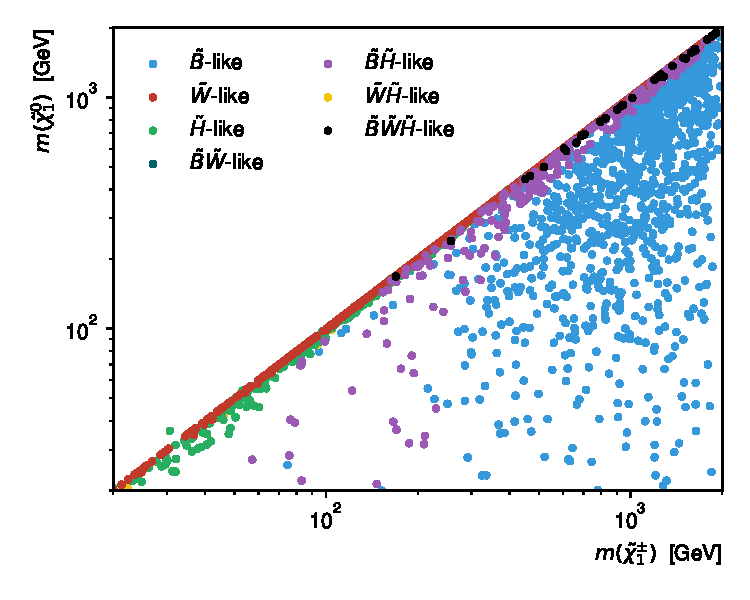
\includegraphics[width=\textwidth]{scatter/lsp_types.pdf}
		\caption{\label{fig:lsp_types}}
	\end{subfigure}\hfill
	\begin{subfigure}[b]{0.5\linewidth}
		\centering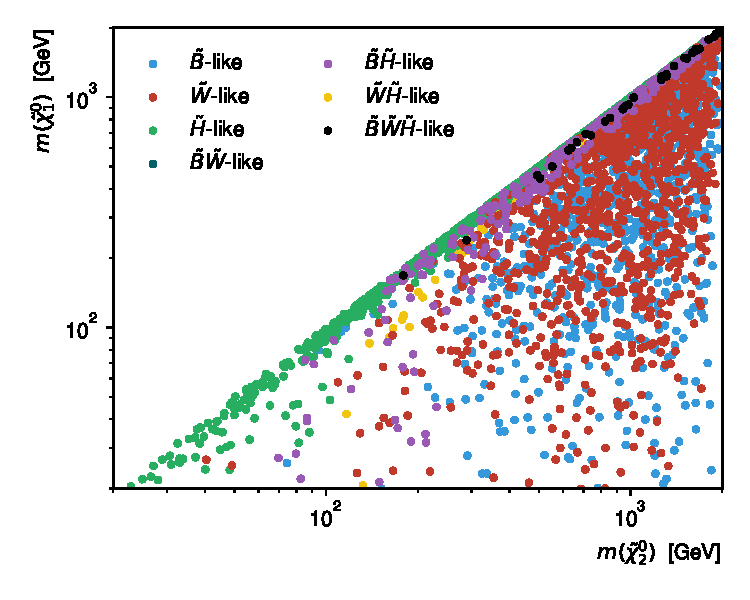
\includegraphics[width=\textwidth]{scatter/lsp_types_N2.pdf}
		\caption{\label{fig:lsp_types_N2}}
	\end{subfigure}\hfill
	\caption{Scatter plot of all models sampled in the \subref{fig:lsp_types} $m(\charg)$--$m(\lsp)$ and \subref{fig:lsp_types_N2} $m(\neutr)$--$m(\lsp)$ planes. The colour encodes the composition of the $\lsp$ in each model. The $\lsp$ is considered to be bino-like ($\tilde{B}$-like), wino-like ($\tilde{W}$-like) or higgsino-like ($\tilde{H}$-like) if the corresponding fraction from the neutralino mass mixing matrix is at least 80\%. Additionally, the $\lsp$ is considered to be of mixed nature if more than one component has a fraction of 20\%. For example, a $\tilde{B}\tilde{W}$-like $\lsp$ has more than 20\% bino and wino components, but less than 20\% higgsino component.}
	\label{fig:lsp_phenomenology}
\end{figure}


The composition of the $\lsp$ in each \gls{pmssm} model sampled is shown in the $m(\charg)$--$m(\lsp)$ and $m(\neutr)$--$m(\lsp)$ planes in~\cref{fig:lsp_types,fig:lsp_types_N2}, respectively. The $\lsp$ is considered to be bino-like ($\tilde{B}$-like), wino-like ($\tilde{W}$-like) or higgsino-like ($\tilde{H}$-like) if the corresponding fraction from the neutralino mass mixing matrix is at least 80\%. If more than one component has a fraction of more than 20\%, then the $\lsp$ is considered to be of mixed nature. The nature of the \gls{lsp} as a function of the mass parameters $M_1$, $M_2$ and $\mu$ is shown as a reference in \cref{fig:lsp_phenomenology_parameters}. 

In the bulk of the $m(\charg)$--$m(\lsp)$ plane, \ie the parameter space targeted by the \onelepton search using the simplified model, a large majority of the models produce a bino-like \gls{lsp} with nearly mass-degenerate $\charg$ and $\neutr$. These models correspond to cases where $M_1 \ll \mu$ and $M_1 < M_2$ and are thus similar to the canonical simplified model considered in the \onelepton search. Some sensitivity can therefore be expected towards these models in the context of the \onelepton search, provided that the branching fractions of the decays $\charg \rightarrow W^\pm \lsp$ and especially $\neutr \rightarrow h \lsp$ are large enough and produce on-shell bosons.

Towards the diagonal of the $m(\charg)$--$m(\lsp)$ plane, \ie for models where the $\charg$ and $\lsp$ are nearly mass-degenerate, the nature of the \gls{lsp} shows a larger variation. In a large set of models where $M_2$ is not too heavy and $M_2 \ll M_1$ as well as $M_2 \ll \mu$, the \gls{lsp} has a significant wino component and is nearly mass-degenerate with the $\charg$, while the $\neutr$ can be more massive. In models where the \gls{lsp} has a large higgsino component, \ie $\mu \ll M_1$ and $\mu \ll M_2$, all three electroweakinos $\charg$, $\neutr$ and $\lsp$ are nearly mass-degenerate and result in very soft decay products, making these models inherently difficult to target.

\section{Impact of the search on the pMSSM}

The impact of the \onelepton search on the \gls{pmssm} is discussed using one-dimensional and two-dimensional distributions in the following sections. A model is considered to be excluded if the observed CL$_s$ value obtained with the simplified likelihood using the smeared truth-level inputs is below 0.05. Of the 5152 models evaluated, the \onelepton search excludes a total of 98, or about 1.9\%, of the models.

For the one-dimensional distributions shown in the following, the total number of models is compared against the number of models excluded by the \onelepton search. An additional pad indicates the ratio between models excluded and total models sampled in each bin of the distribution. In the two-dimensional distributions, the numbers in the bins indicate the number of \gls{pmssm} models falling into each bin. In these distributions, the fraction of models excluded with the \onelepton search is encoded using the $z$-axis, represented by a colour bar. Bins in which all models are excluded are coloured in black, while bins without any excluded models are left white. Where applicable, the exclusion contour obtained by the \onelepton search using the simplified model is overlaid.

\subsection{Impact on electroweakino masses}\label{sec:impact_electroweakino_masses}

 \begin{figure}
	\centering
	\begin{subfigure}[b]{0.5\linewidth}
		\centering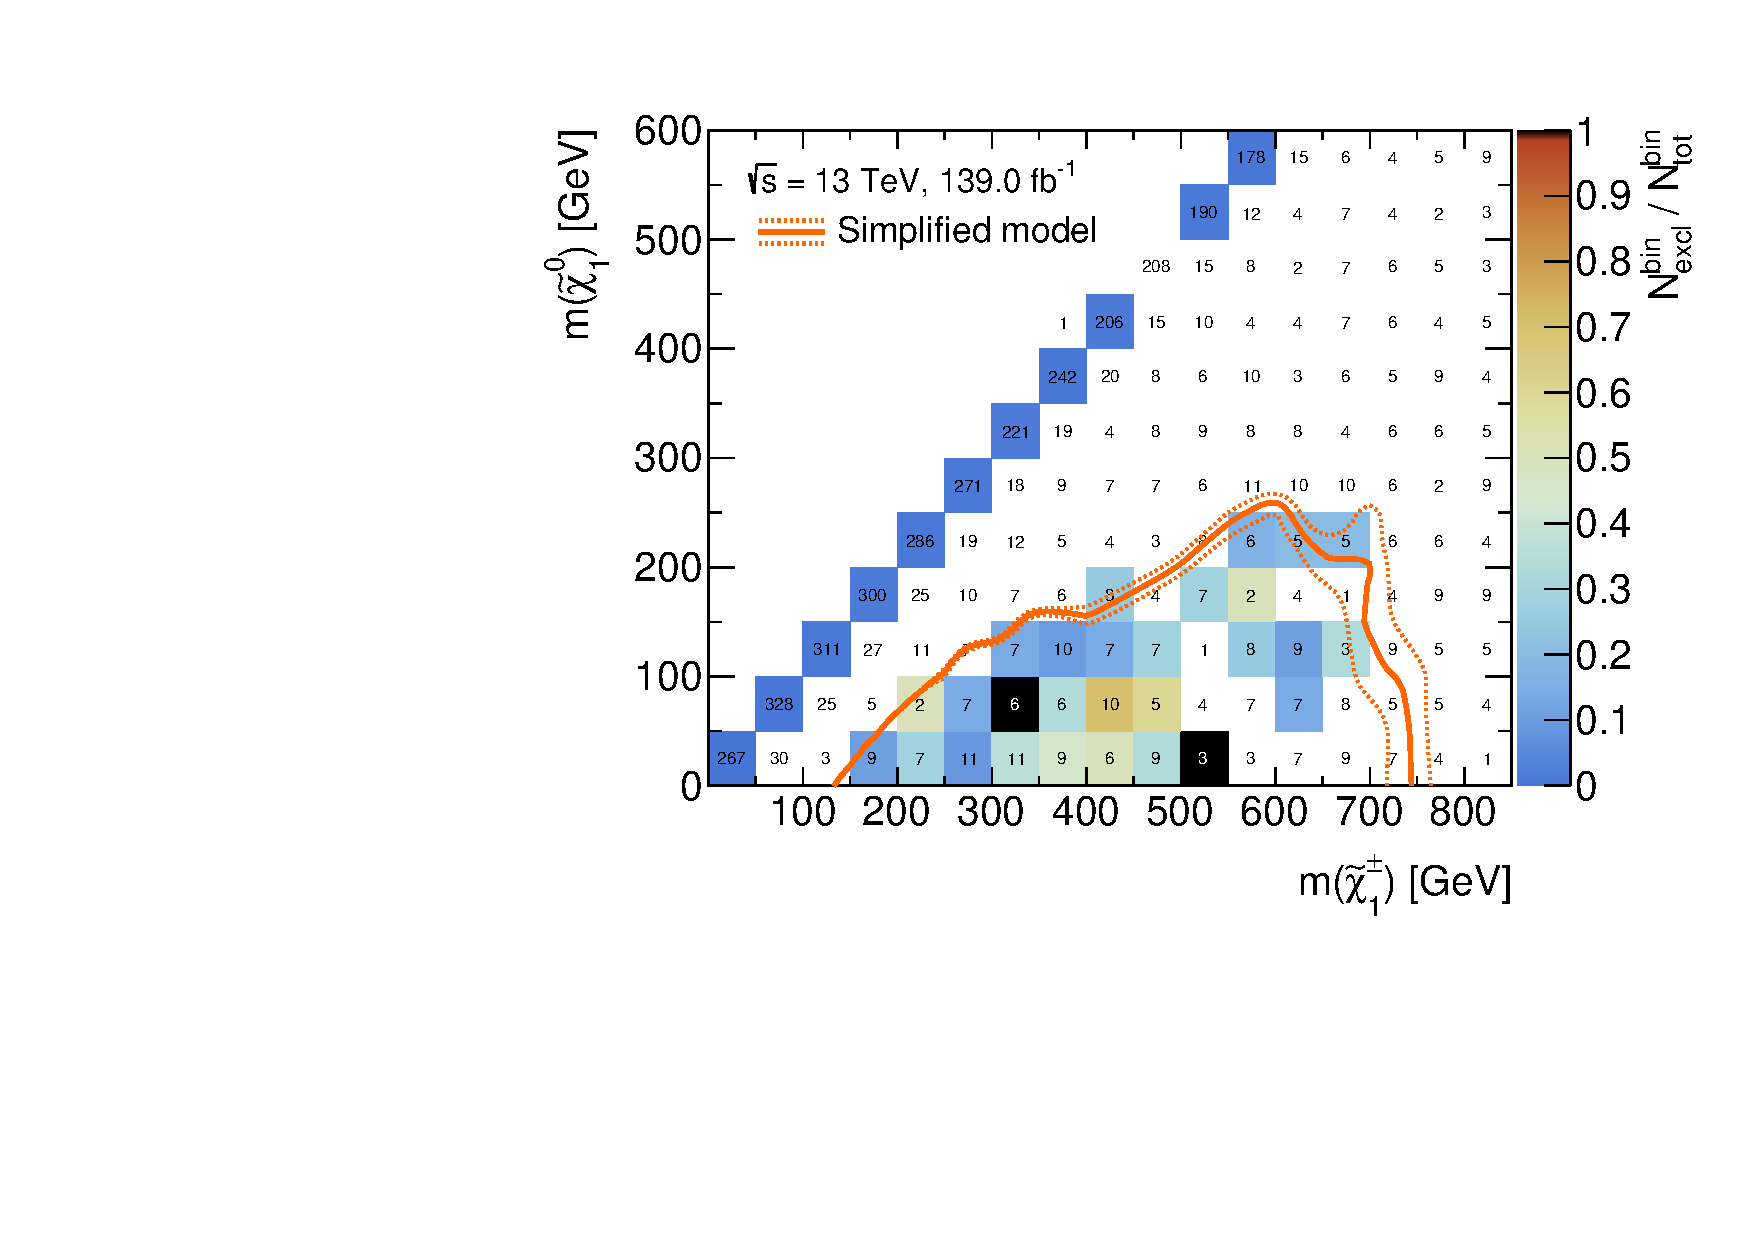
\includegraphics[width=\textwidth]{cut_none/mchi1p_mlsp_contour}
		\caption{\label{fig:mchi1p_mlsp_contour}}
	\end{subfigure}\hfill
	\begin{subfigure}[b]{0.5\linewidth}
		\centering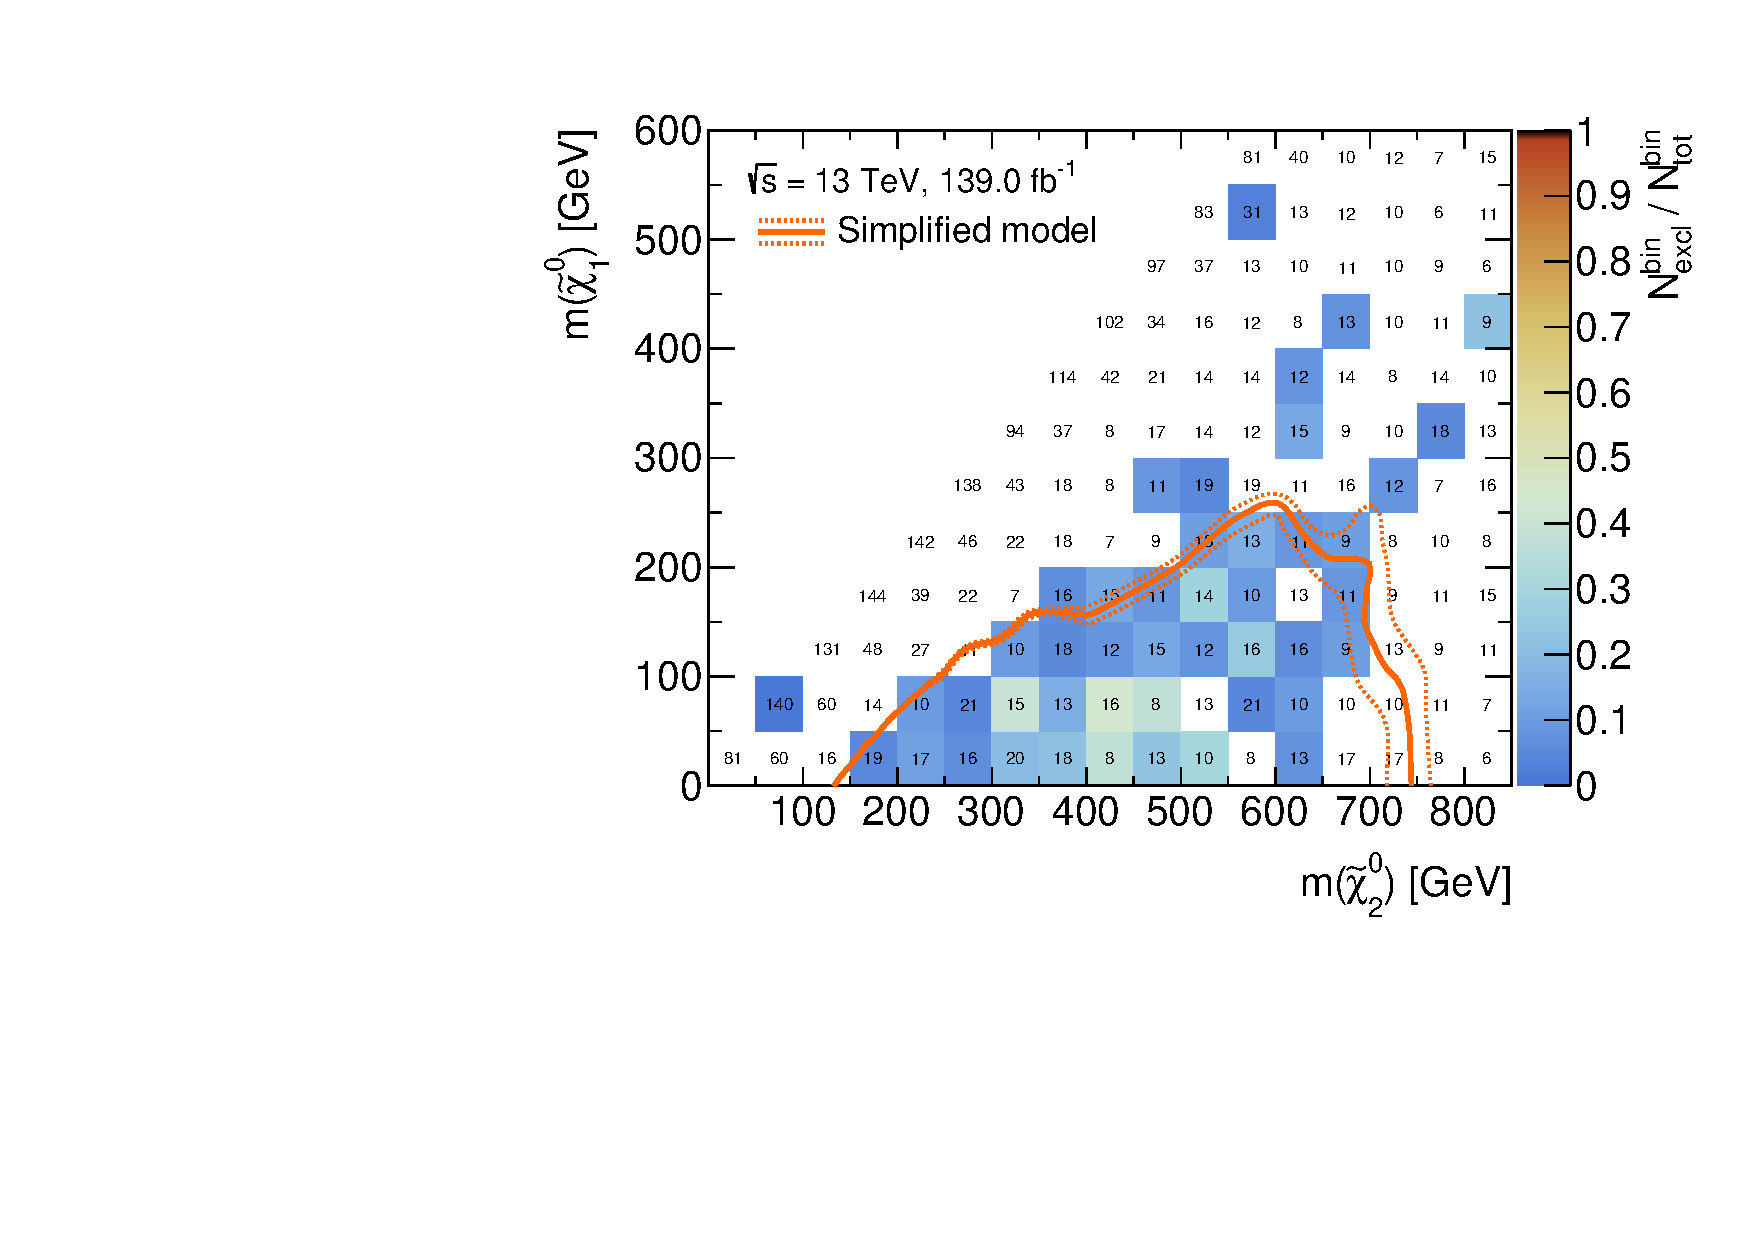
\includegraphics[width=\textwidth]{cut_none/mchi20_mlsp_contour}
		\caption{\label{fig:mchi20_mlsp_contour}}
	\end{subfigure}\hfill
	\begin{subfigure}[b]{0.5\linewidth}
		\centering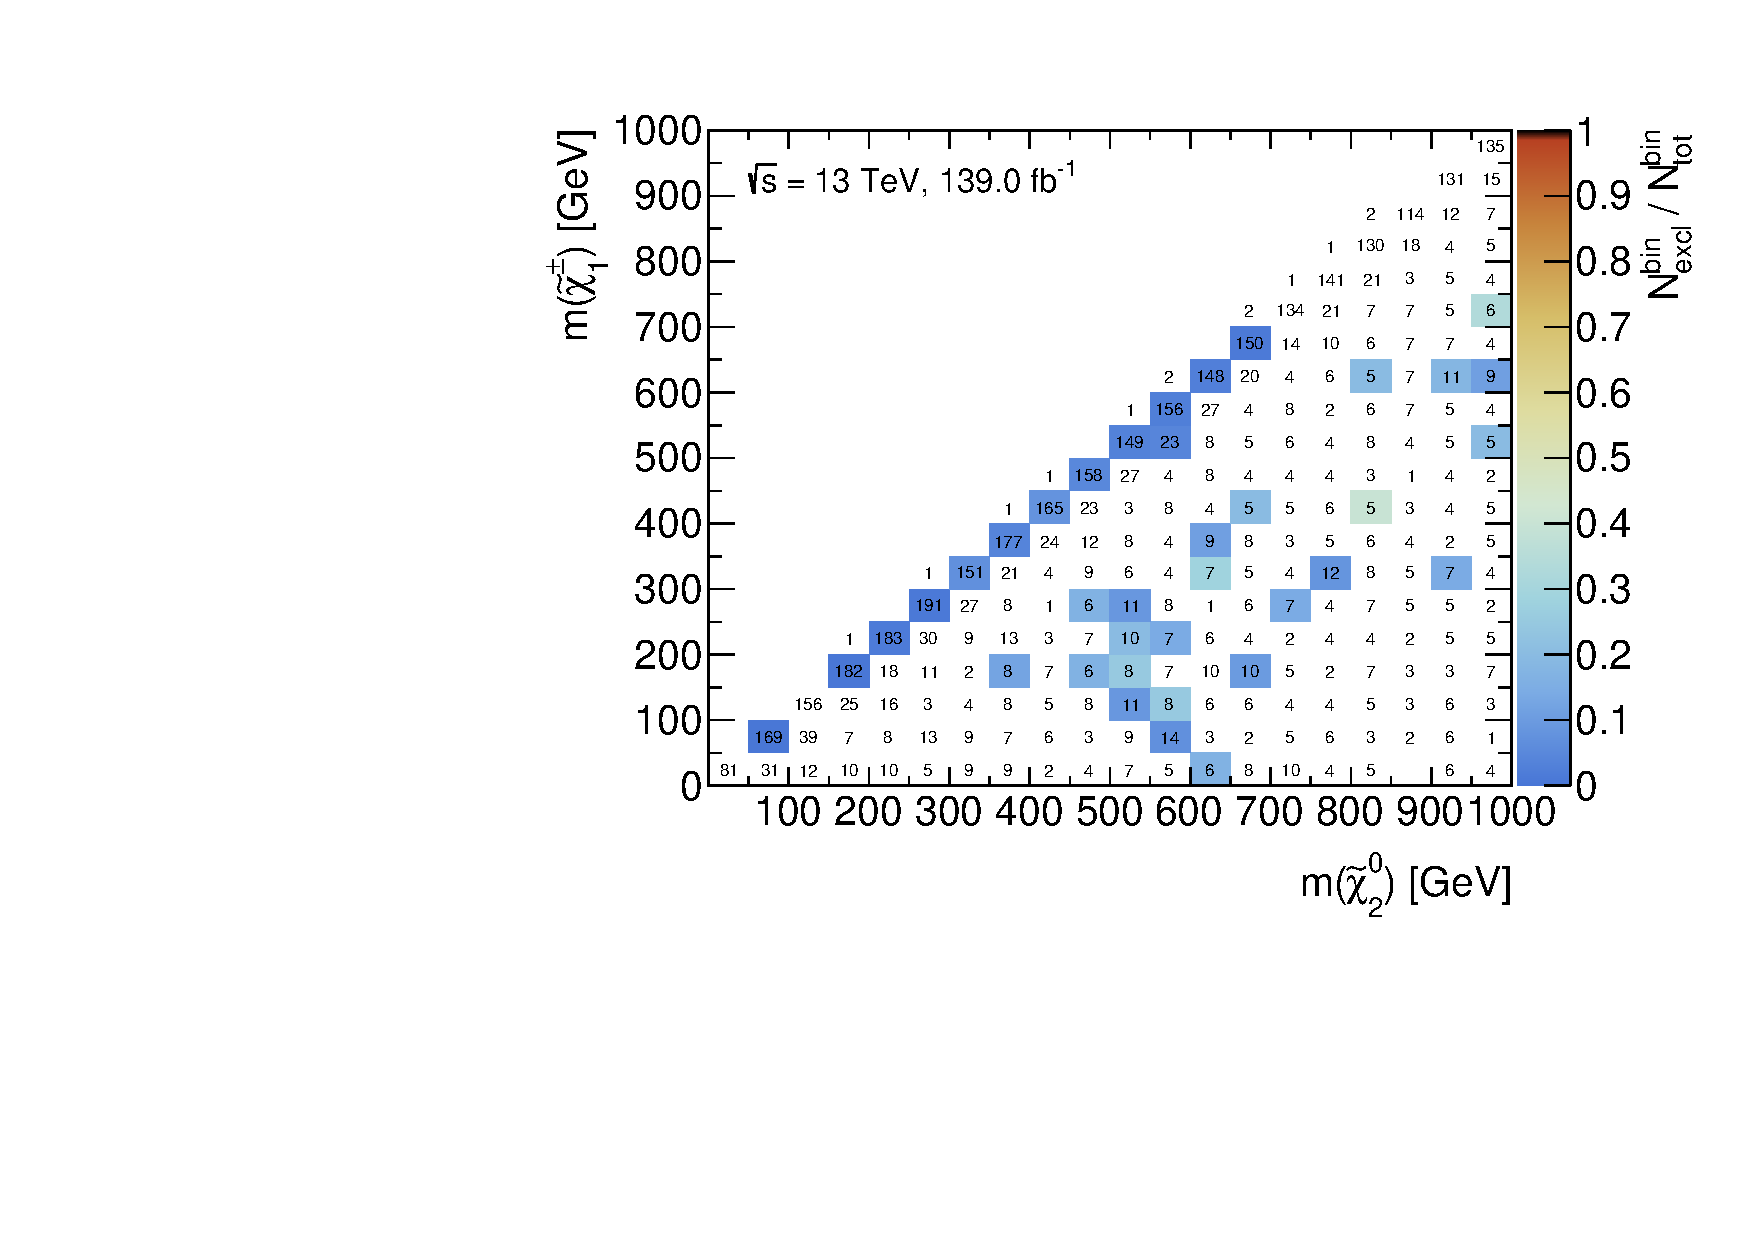
\includegraphics[width=\textwidth]{cut_none/mchi1p_mchi20_contour}
		\caption{\label{fig:mchi1p_mchi20_contour}}
	\end{subfigure}\hfill
	\caption{Bin-by-bin fraction of excluded models as a function of the relevant sparticle masses. The numbers in the bins correspond to the total number of models sampled falling into the respective bin. The number of models excluded by the \onelepton search is encoded with a colour bar ranging from 0 to 1. Where all models in a given bin are excluded, the bin is coloured in black. Bins without any models excluded are left white. Models are evaluated using the simplified likelihood of the \onelepton search. The simplified model contour is shown in orange.}
	\label{fig:impact_electroweakinos_2D}
\end{figure}


 \begin{figure}
	\centering
	\begin{subfigure}[b]{0.5\linewidth}
		\centering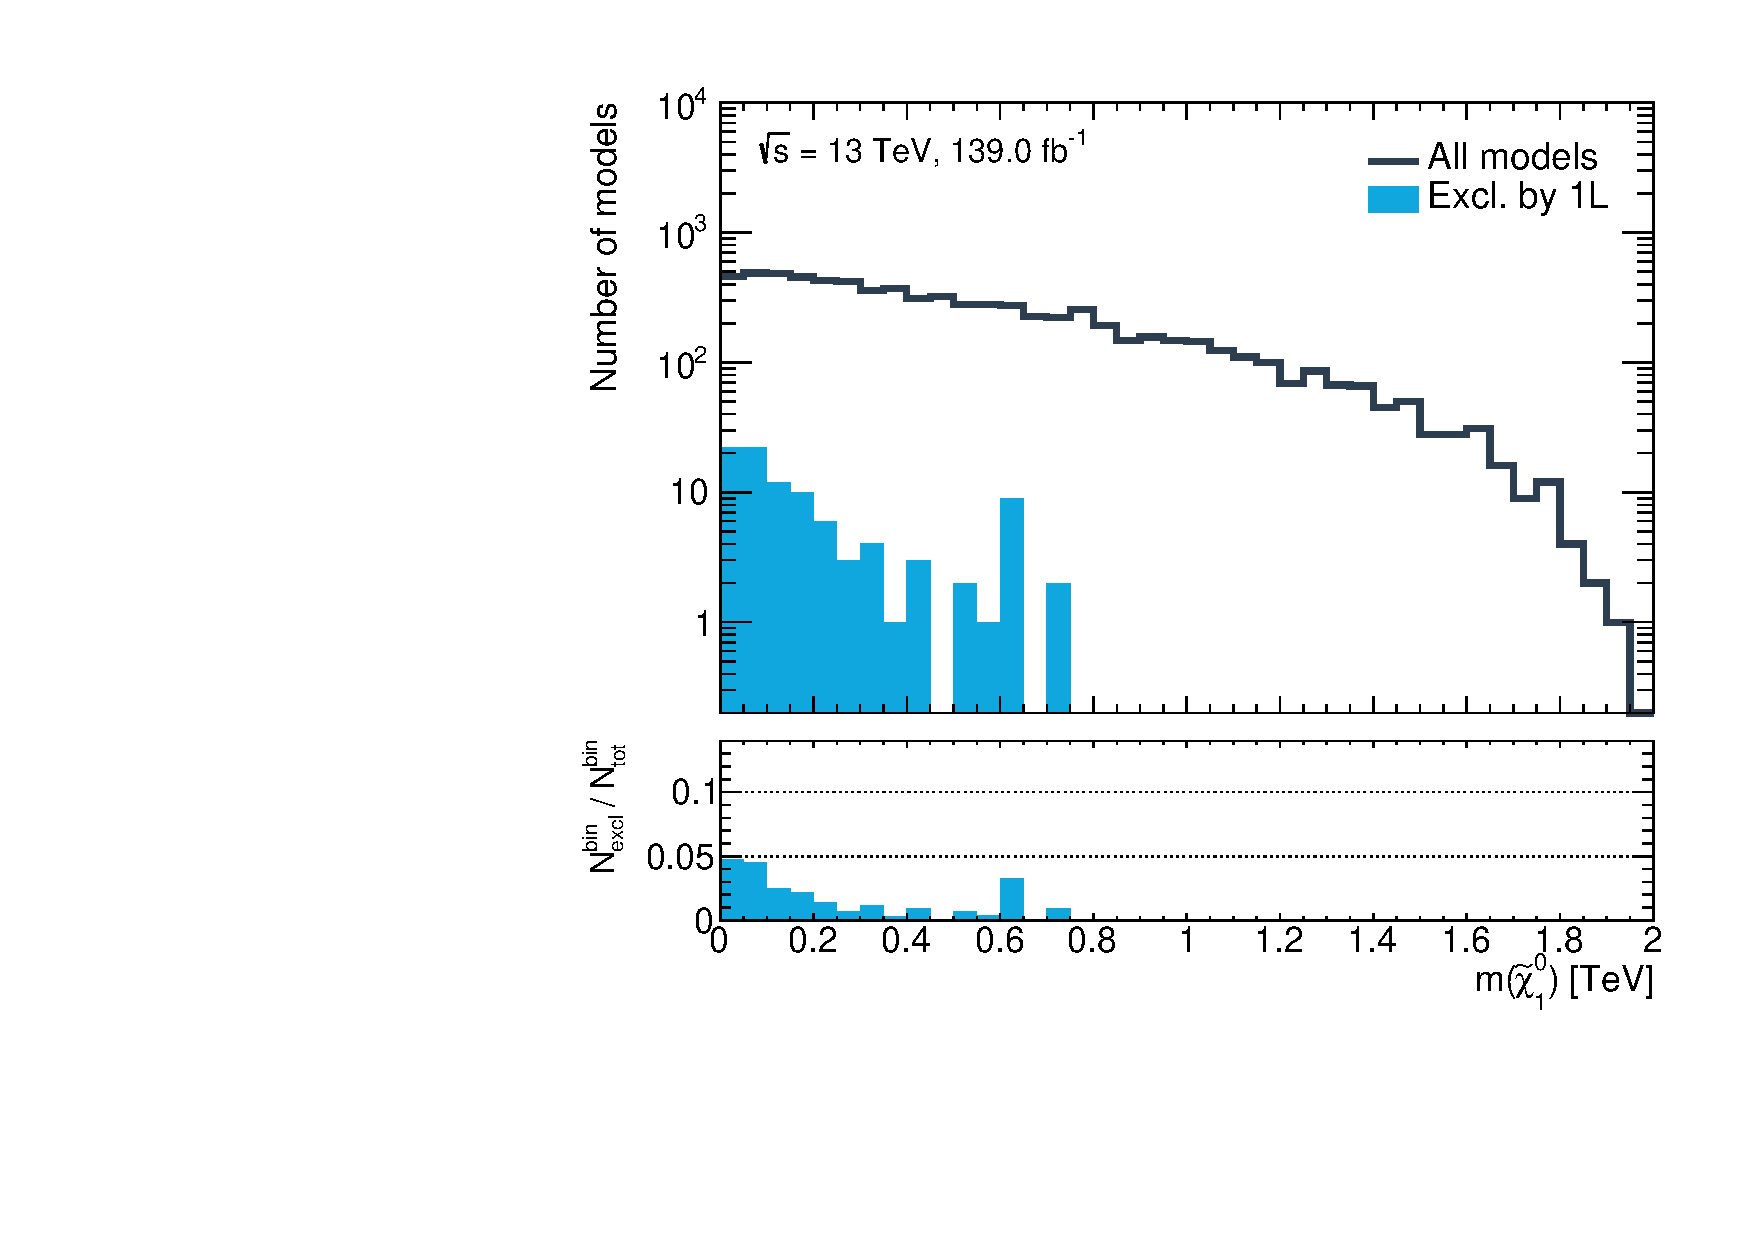
\includegraphics[width=\textwidth]{1D/m_chi_10}
	\end{subfigure}\hfill
	\begin{subfigure}[b]{0.5\linewidth}
		\centering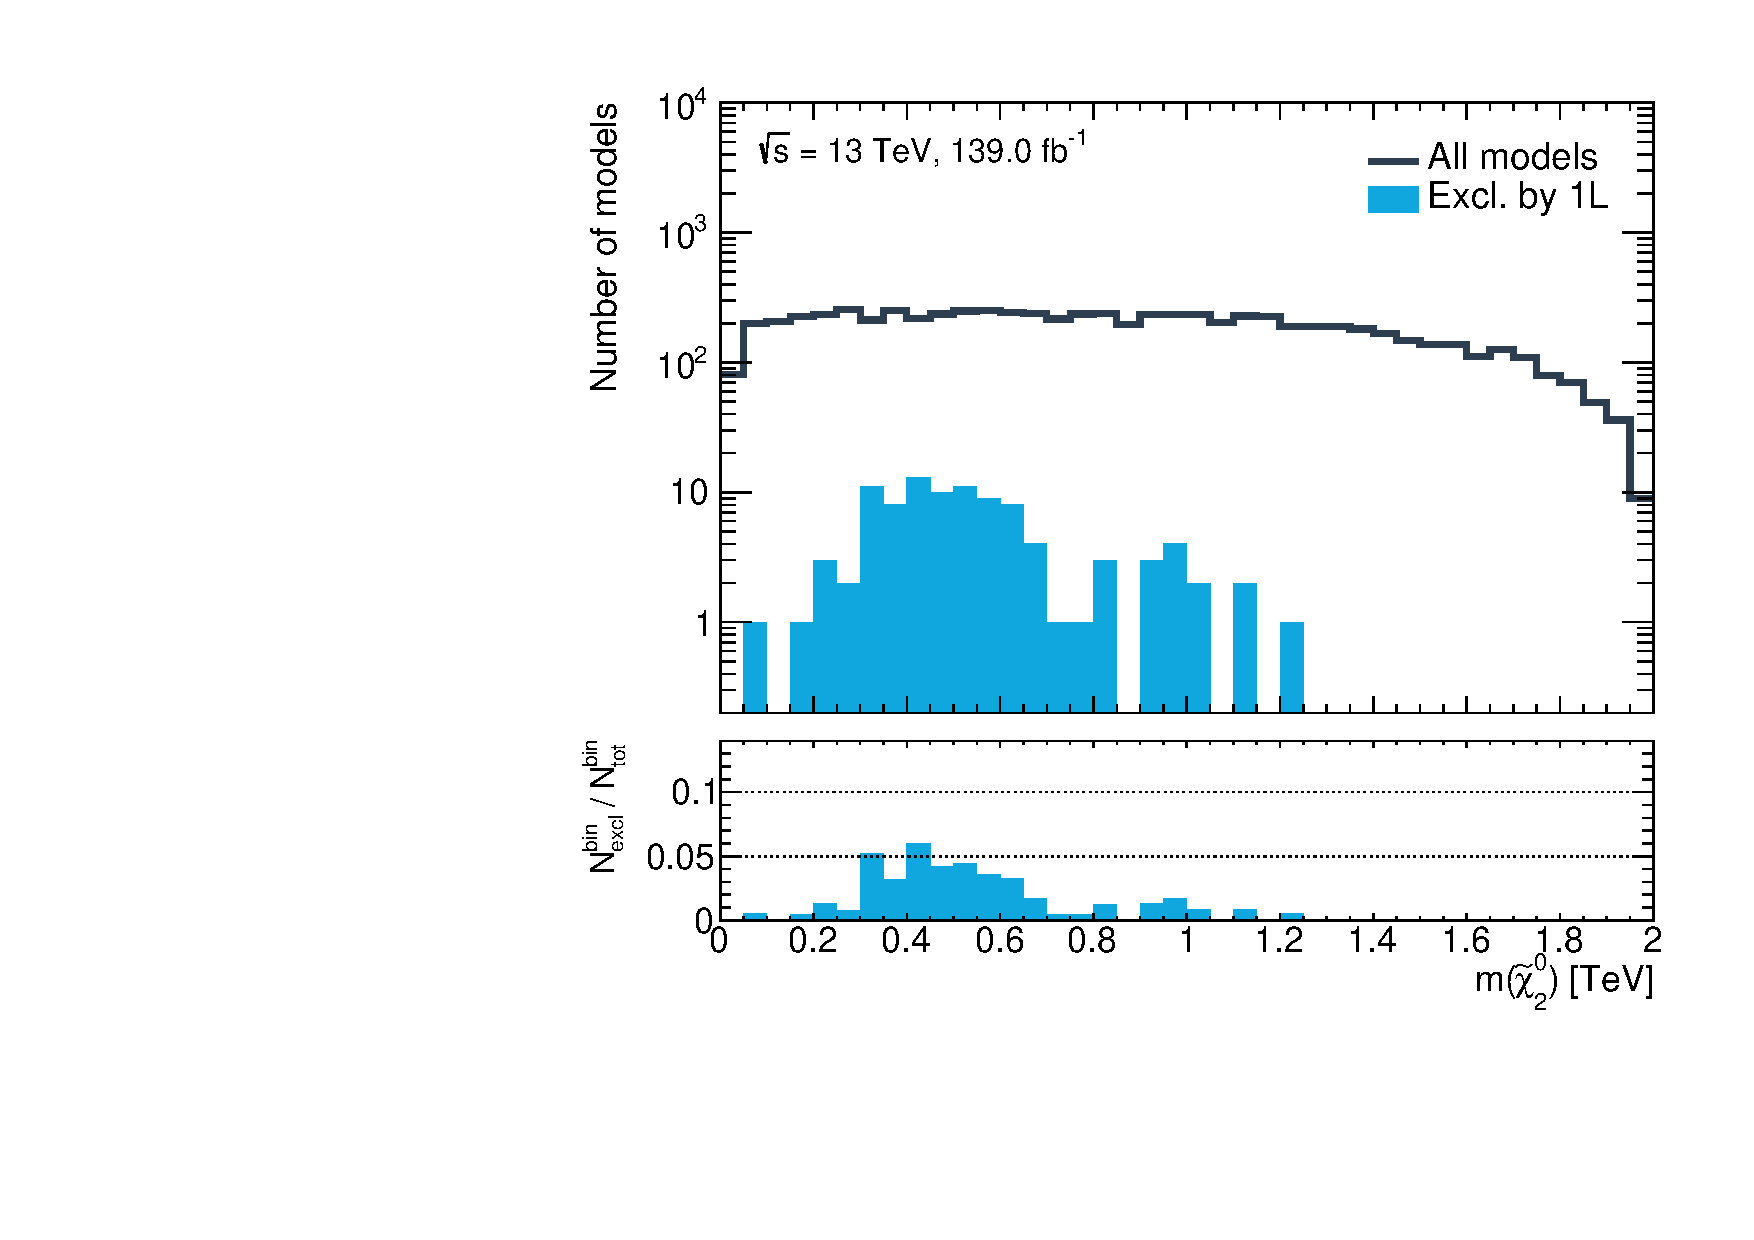
\includegraphics[width=\textwidth]{1D/m_chi_20}
	\end{subfigure}\hfill
	\begin{subfigure}[b]{0.5\linewidth}
		\centering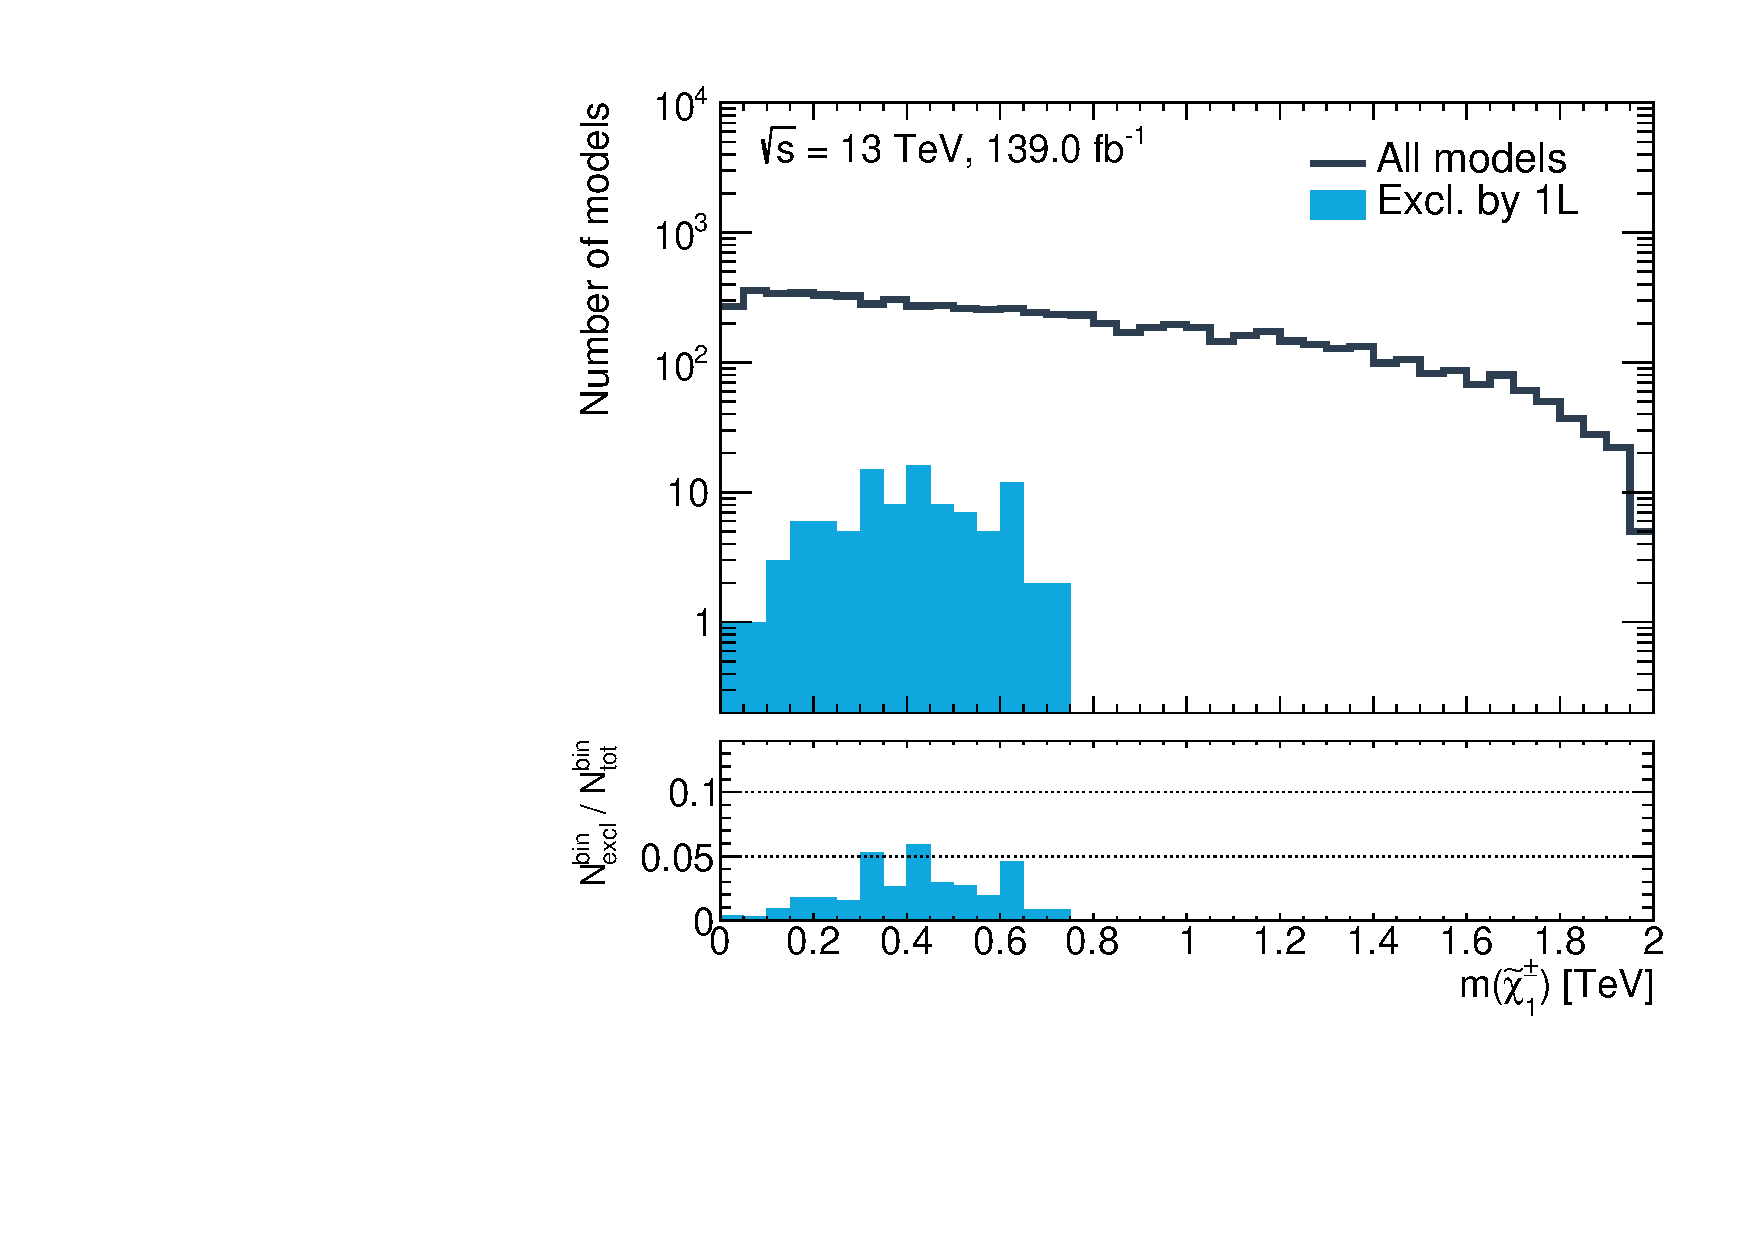
\includegraphics[width=\textwidth]{1D/m_chi_1p}
	\end{subfigure}\hfill
	\caption{Bin-by-bin number of excluded models as a one-dimensional function of the electroweakino masses. The bin-wise fraction of excluded models, $N^\mathrm{bin}_\mathrm{excl} / N^\mathrm{bin}_\mathrm{total}$, is shown in the lower pad. All models are evaluated using the simplified likelihood of the \onelepton search.}
	\label{fig:impact_electroweakinos_1D}
\end{figure}


\Cref{fig:impact_electroweakinos_2D,fig:impact_electroweakinos_1D} show the bin-by-bin fractions of models excluded by the \onelepton search as two- and one-dimensional distributions, respectively. From the $\charg$--$\lsp$ plane in \cref{fig:mchi1p_mlsp_contour}, it can be seen that the \onelepton search is most sensitive to \gls{pmssm} models in mass ranges similar to those excluded in the context of the simplified model. Most of the models excluded have $\charg$/$\neutr$ masses ranging from roughly $\SI{200}{\GeV}$ to about $\SI{700}{\GeV}$ and \gls{lsp} ranging masses from $\SI{0}{\GeV}$ to about $\SI{300}{\GeV}$. The proportion of excluded models peaks at $m(\charg,\neutr) \approx \SI{450}{\GeV}$ and light \glspl{lsp} with $\lsp < \SI{150}{\GeV}$, as visible in~\cref{fig:impact_electroweakinos_1D}. 

The models excluded by the \onelepton search can roughly be classified in two categories: models lying within the simplified model exclusion contour and models with nearly mass-degenerate $\charg$ and $\neutr$. As discussed in \cref{sec:lsp_pheno}, most models within the simplified model exclusion contour produce a bino-like \gls{lsp} and result in nearly mass-degenerate $\charg$ and $\neutr$. \Cref{fig:impact_electroweakinos_2D_bino_lsp} illustrates this behaviour further. Expectedly, the \onelepton search shows sensitivity to $\charg\neutr$ production in models with wino-like electroweakinos and a bino-like $\lsp$, resulting in spectra close to that of the canonical simplified model signature originally considered in the search. 

The second category of models excluded comprises cases where the \gls{lsp} is wino-like and nearly mass-degenerate with the $\charg$, corresponding to the diagonal in~\cref{fig:mchi1p_mlsp_contour}. As the mass difference between the \gls{lsp} and the $\charg$ is typically of the order of a few $\SI{100}{\MeV}$, the $\charg$ becomes long-lived, and primarily decays to a \gls{lsp} and an off-shell \textit{W} boson decaying into soft objects not reconstructed in the detector.
If the $\charg$ is produced with large momentum, it can live long enough to traverse multiple layers of the ATLAS pixel detector before decaying, leading to a disappearing track signature. Searches targeting prompt electroweakino decays are not expected to be sensitive to these models, and instead dedicated disappearing track searches are developed within ATLAS (cf. \eg \reference\cite{ATLAS-CONF-2021-015}). 
Even though no sensitivity to these models is expected from the \onelepton search, a small set of models with a wino-like \gls{lsp} can still be excluded. These models correspond to scenarios where the $\tilde{\chi}^\pm_2$ is not too heavy such that the \onelepton search is sensitive to $\tilde{\chi}^\pm_2\neutr$ production with cross sections of $\mathcal{O}(\SI{1}{\femto\barn})$.
If the $\tilde{\chi}^\pm_2$ decays directly into the \gls{lsp} via $\tilde{\chi}^\pm_2 \rightarrow W^\pm \lsp$, enough events with an isolated lepton can occur, allowing to exclude the model.

No sensitivity is observed for \gls{pmssm} models with higgsino-like electroweakinos, \ie compressed mass spectra. This is expected, as the electroweakino decays in such scenarios typically produce off-shell \textit{W}, \textit{Z} and \textit{h} bosons, resulting in very soft final state objects the \onelepton search is not optimised for. Dedicated searches (see \eg \reference\cite{SUSY-2018-16}) exist in ATLAS to target such compressed scenarios and work is ongoing to include these in the scans of the \gls{pmssm}.

 \begin{figure}
	\centering
	\begin{subfigure}[b]{0.5\linewidth}
		\centering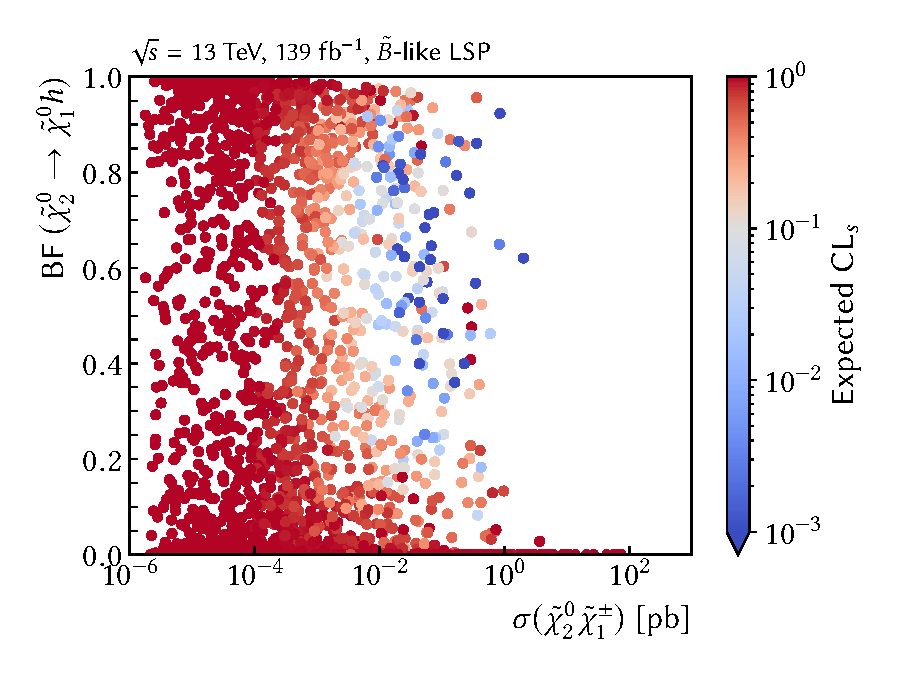
\includegraphics[width=\textwidth]{scatter/fig_scatter_xsec_BFHiggs_bino}
		\caption{\label{fig:fig_scatter_xsec_BFHiggs_bino}}
	\end{subfigure}\hfill
	\begin{subfigure}[b]{0.5\linewidth}
		\centering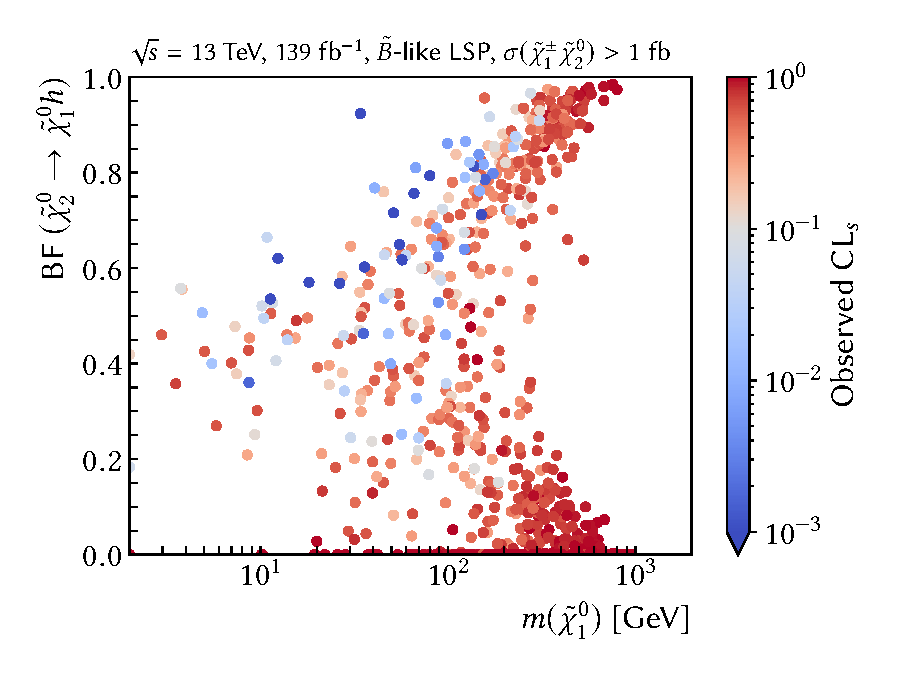
\includegraphics[width=\textwidth]{scatter/fig_scatter_mchi10_BFHiggs_bino_withXsecCut}
		\caption{\label{fig:fig_scatter_mchi10_BFHiggs_bino_withXsecCut}}
	\end{subfigure}\hfill
	\caption{Density of the \gls{pmssm} models with bino-like $\lsp$ projected onto the plane spanned by \subref{fig:fig_scatter_xsec_BFHiggs_bino} $\charg\neutr$ pair-production cross section and $\mathrm{BF}(\neutr \rightarrow h \lsp)$ and \subref{fig:fig_scatter_mchi10_BFHiggs_bino_withXsecCut} $m(\lsp)$ and $\mathrm{BF}(\neutr \rightarrow h \lsp)$. The observed CL$_s$ value obtained for each model using the \onelepton search is encoded using the colour-palette. Models with a red tint cannot be excluded, models with a neutral white tint are on the boundary of exclusion, and models with a blue tint can be excluded. Only models satisfying $\sigma(\charg\neutr)>\SI{1}{\femto\barn}$ are shown in fig.~\subref{fig:fig_scatter_mchi10_BFHiggs_bino_withXsecCut}.}
	\label{fig:bino_sensitivity}
\end{figure}

In general, the sensitivity to \gls{pmssm} models is significantly reduced compared to the simplified model exclusion contour, even in the parameter space generating models with spectra similar to that of the simplified model. The crucial difference, responsible for the loss in sensitivity, is the fact that the simplified model assumes branching ratios of 100\% of the $\charg \rightarrow W^\pm \lsp$ and $\neutr \rightarrow h \lsp$ decays (with on-shell \textit{W} and \textit{h} bosons).
While the former is in general a good assumption in \gls{pmssm} models where $m(\lsp)+m(W) \lesssim m(\charg)\lesssim m(\neutr)$, the latter turns out not to be the dominant decay of the $\neutr$ in many models where the decay $\neutr \rightarrow Z \lsp$ dominates instead.
The couplings of the $\neutr$ to the Higgs boson are suppressed by powers of $\vert\mu\vert/M_2$ in the gaugino-like regions~\cite{Arbey:2012fa}, meaning that the branching fraction of $\neutr \rightarrow h \lsp$ takes on reasonably high values only in models with an \gls{lsp} containing a substantial bino component.
The Higgs coupling suppression is illustrated in \cref{fig:higgs_coupling_neutralino}. As can be seen from~\cref{fig:mchi1p_mlsp_contour}, even in the bulk of the $\charg$--$\lsp$ plane---containing mostly models with a bino-like \gls{lsp}---not all models can be excluded by the simplified \onelepton search.
\Cref{fig:bino_sensitivity} shows that many of these models have either a small $\charg\neutr$ pair-production cross section or low values for $\mathrm{BF}(\neutr \rightarrow h \lsp)$, meaning that either not enough events are produced in the first place (because the electroweakinos are too heavy), or not enough Higgs candidates can be reconstructed.
For the few non-excluded models with reasonably high $\charg\neutr$ pair-production cross section $\sigma(\charg\neutr) \gtrsim\SI{1}{\femto\barn}$ and high enough Higgs coupling to $\neutr$, the mass of the \gls{lsp} turns out to be too high ($m(\lsp)\gtrsim \SI{300}{\GeV}$), typically resulting in final states with insufficient $\etmiss$ and soft objects in the context of the \onelepton search.  

As a cross-check, a significant portion of the models with bino-like \gls{lsp} were reprocessed with $\mathrm{BF}(\neutr \rightarrow h \lsp)$ fixed to unity (and $\mathrm{BF}(\neutr \rightarrow Z \lsp)$ consequently set to disappear) and subsequently reanalysed with the \onelepton search.
\Cref{fig:mchi1p_mchi20_contour_bino_lsp_wh_only} reveals that significantly more models can be excluded within the simplified model contour when the simplified model branching fraction assumption is restored. As the $\neutr$ decay into a $Z$ boson and $\lsp$ is the competing decay to $\neutr \rightarrow h \lsp$, statistically combining searches targeting these decay modes could recover the loss in sensitivity. Likewise, the development of searches targeting both decay modes at the same time, would also recover the full sensitivity\footnote{Provided that they are targeted with disjoint signal regions such that a combined likelihood can be built.}.  

\begin{figure}
	\centering
	\begin{subfigure}[b]{0.49\linewidth}
		\centering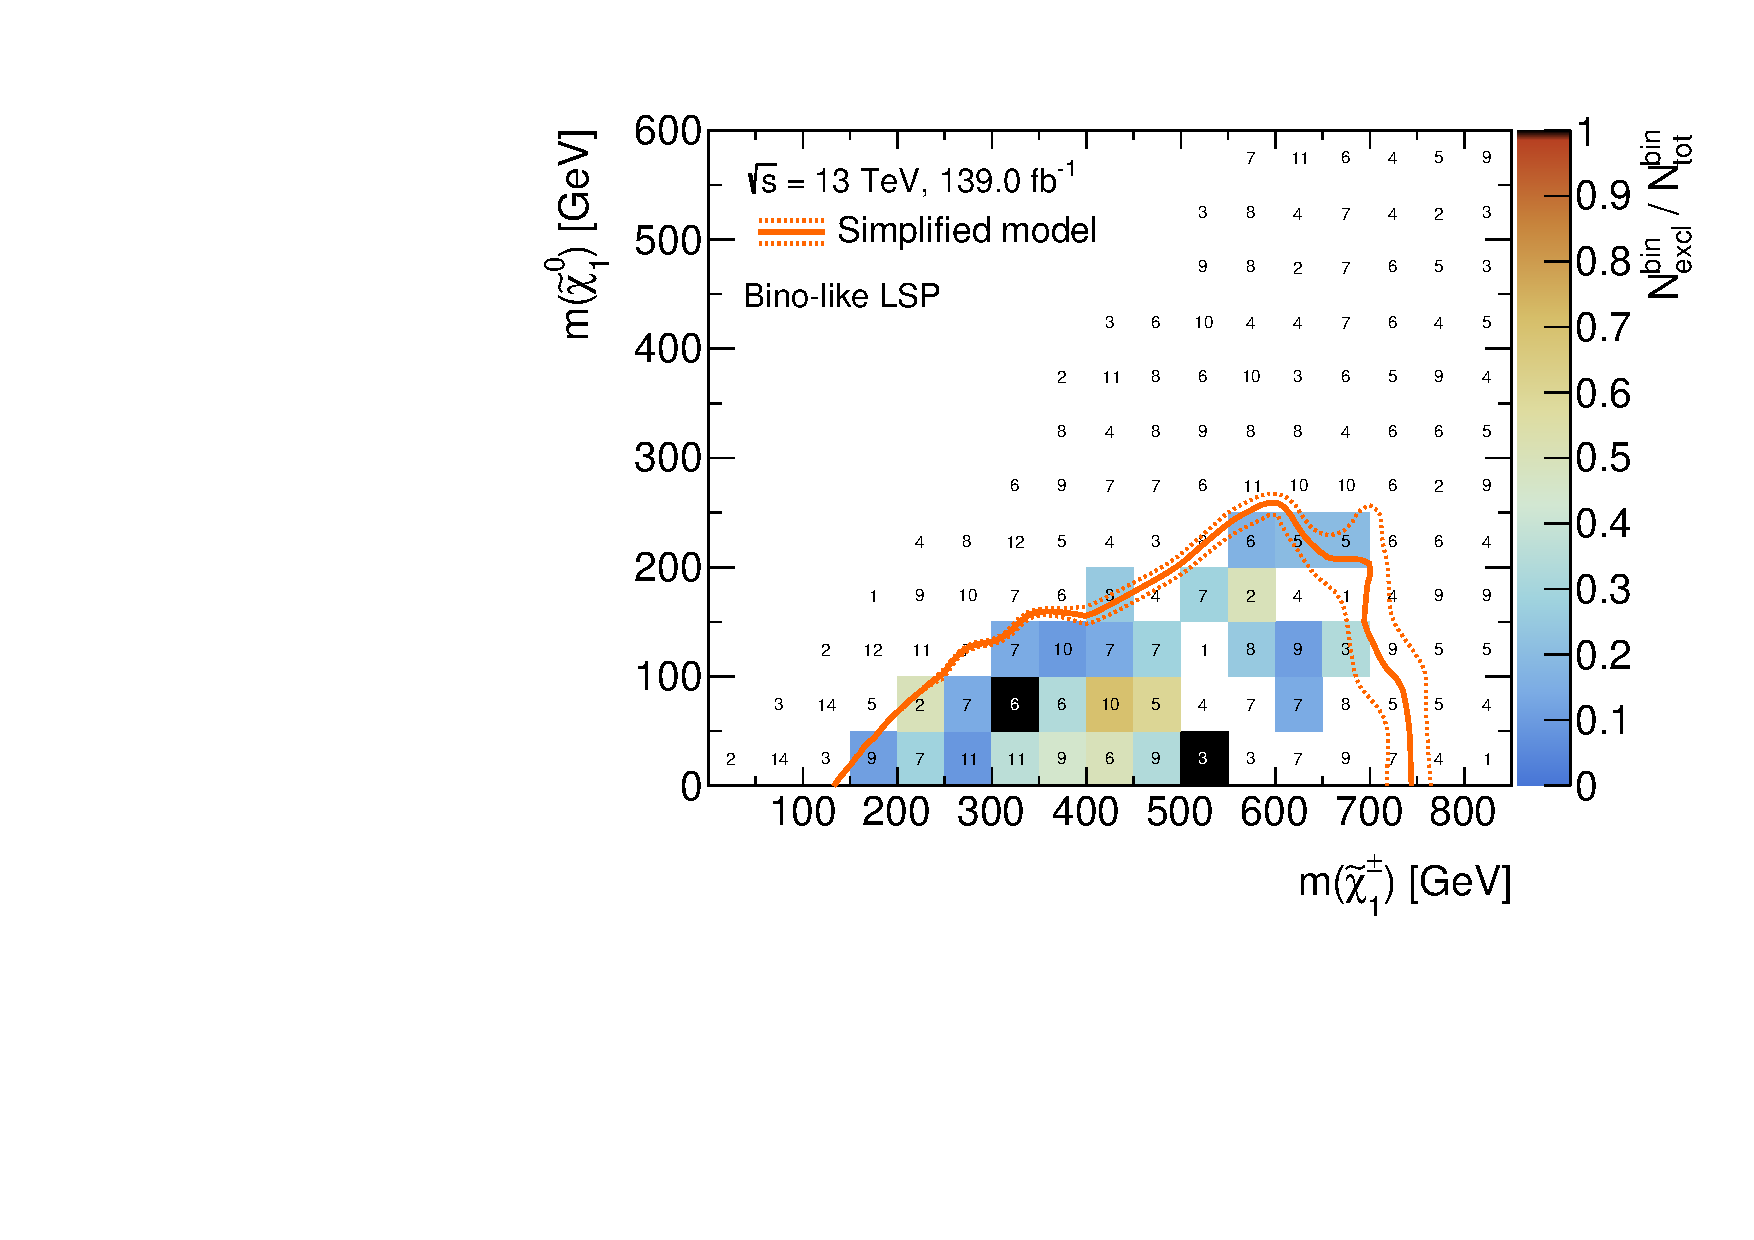
\includegraphics[width=\textwidth]{cut_bino_LSP/mchi1p_mlsp_contour}
		\caption{Mixed BFs\label{fig:mchi1p_mchi20_contour_bino_lsp_orig}}
	\end{subfigure}\hfill
	\begin{subfigure}[b]{0.49\linewidth}
		\centering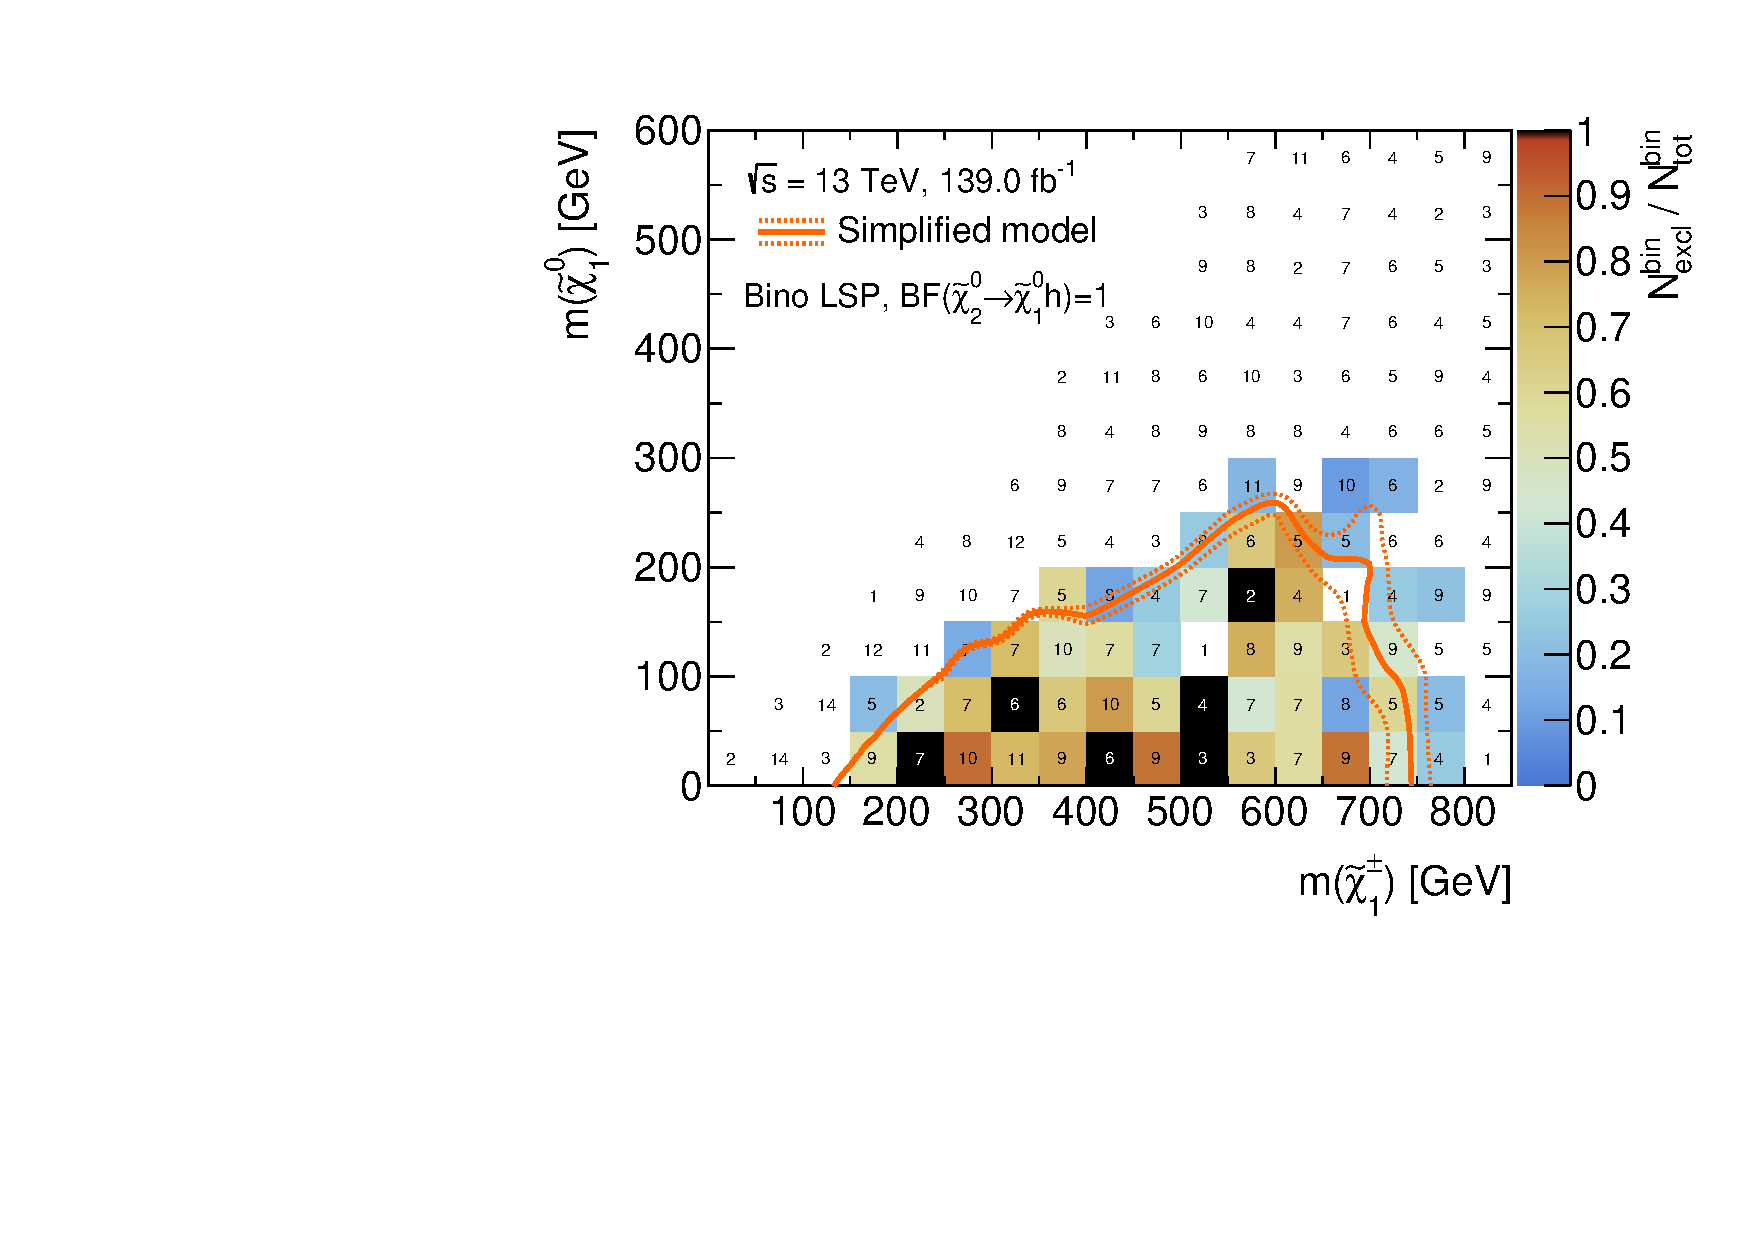
\includegraphics[width=\textwidth]{cut_none_bino_LSP_Wh-only/mchi1p_mlsp_contour}
		\caption{$\mathrm{BF}(\neutr \rightarrow h \lsp) = 1$\label{fig:mchi1p_mchi20_contour_bino_lsp_wh_only}}
	\end{subfigure}\hfill
	\caption{Bin-by-bin fraction of excluded models with a bino-like $\lsp$ as a function of $m(\charg)$ and $m(\lsp)$. In fig.~\subref{fig:mchi1p_mchi20_contour_bino_lsp_orig} the \gls{pmssm} models originally sampled are shown. In fig~\subref{fig:mchi1p_mchi20_contour_bino_lsp_wh_only}, the $\mathrm{BF}(\neutr \rightarrow h \lsp)$ is hard-coded to 100\% after which event generation  and \onelepton analysis evaluation are re-exectued. Only models with a bino-like \gls{lsp} are shown.}
	\label{fig:mixed_BFs}
\end{figure}

\subsection{Impact on pMSSM parameters}

\begin{figure}
	\centering
	\begin{subfigure}[b]{0.5\linewidth}
		\centering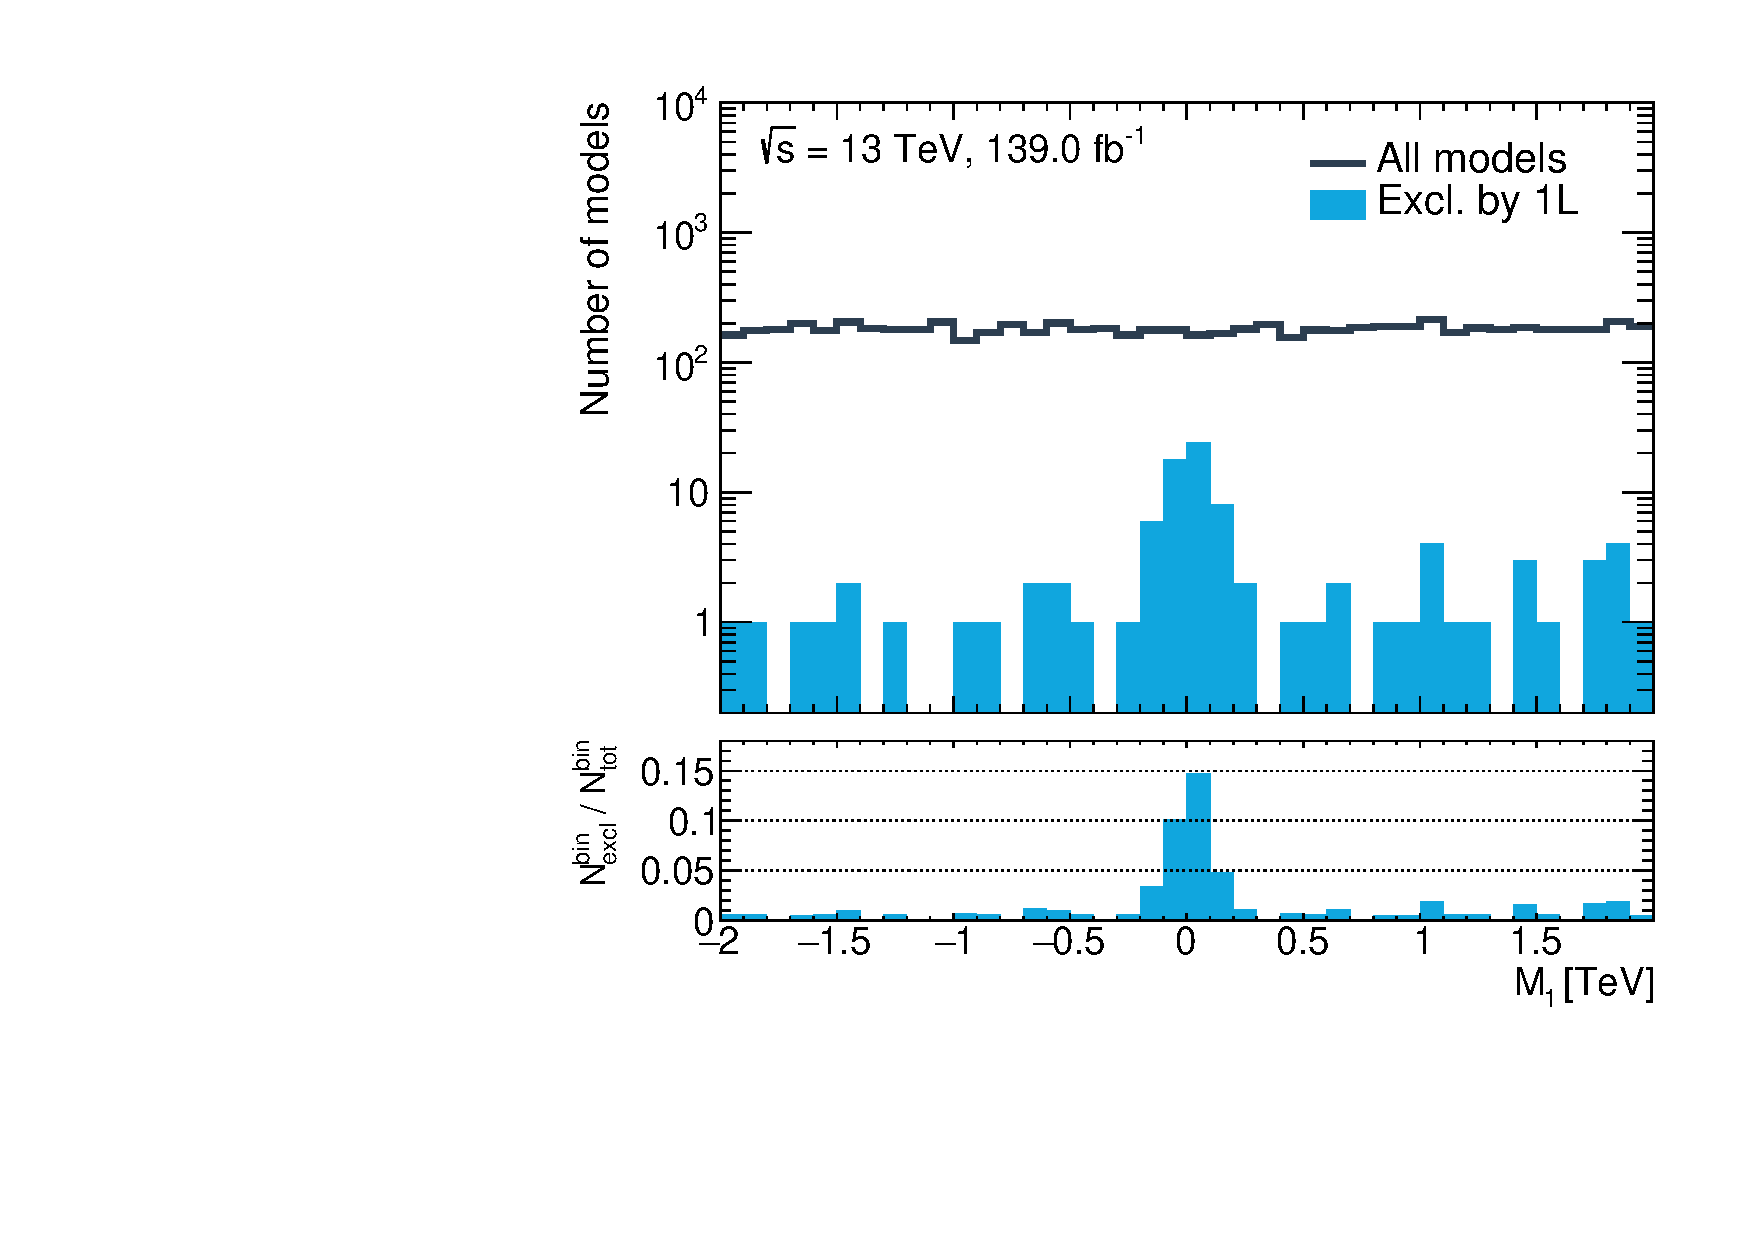
\includegraphics[width=\textwidth]{1D/M1}
	\end{subfigure}\hfill
	\begin{subfigure}[b]{0.5\linewidth}
		\centering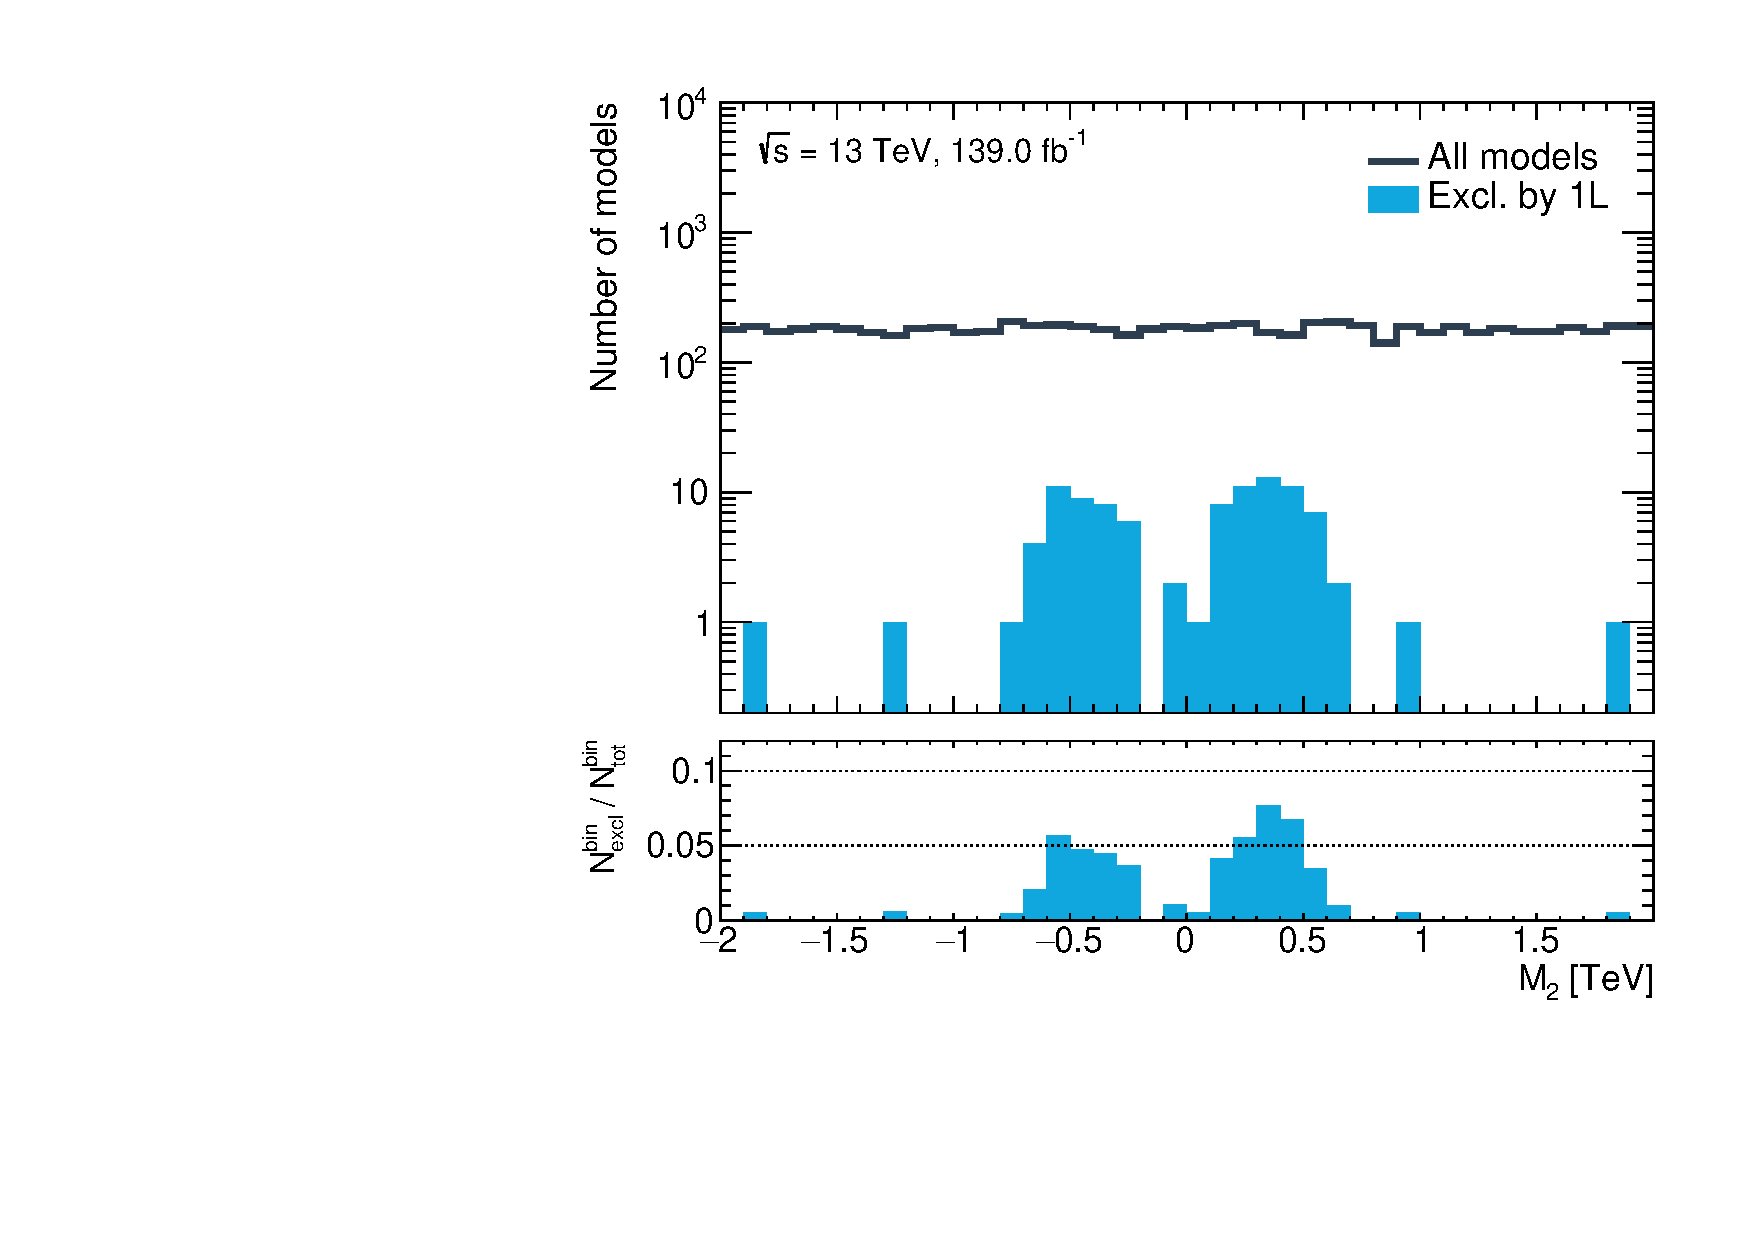
\includegraphics[width=\textwidth]{1D/M2}
	\end{subfigure}\hfill
	\begin{subfigure}[b]{0.5\linewidth}
		\centering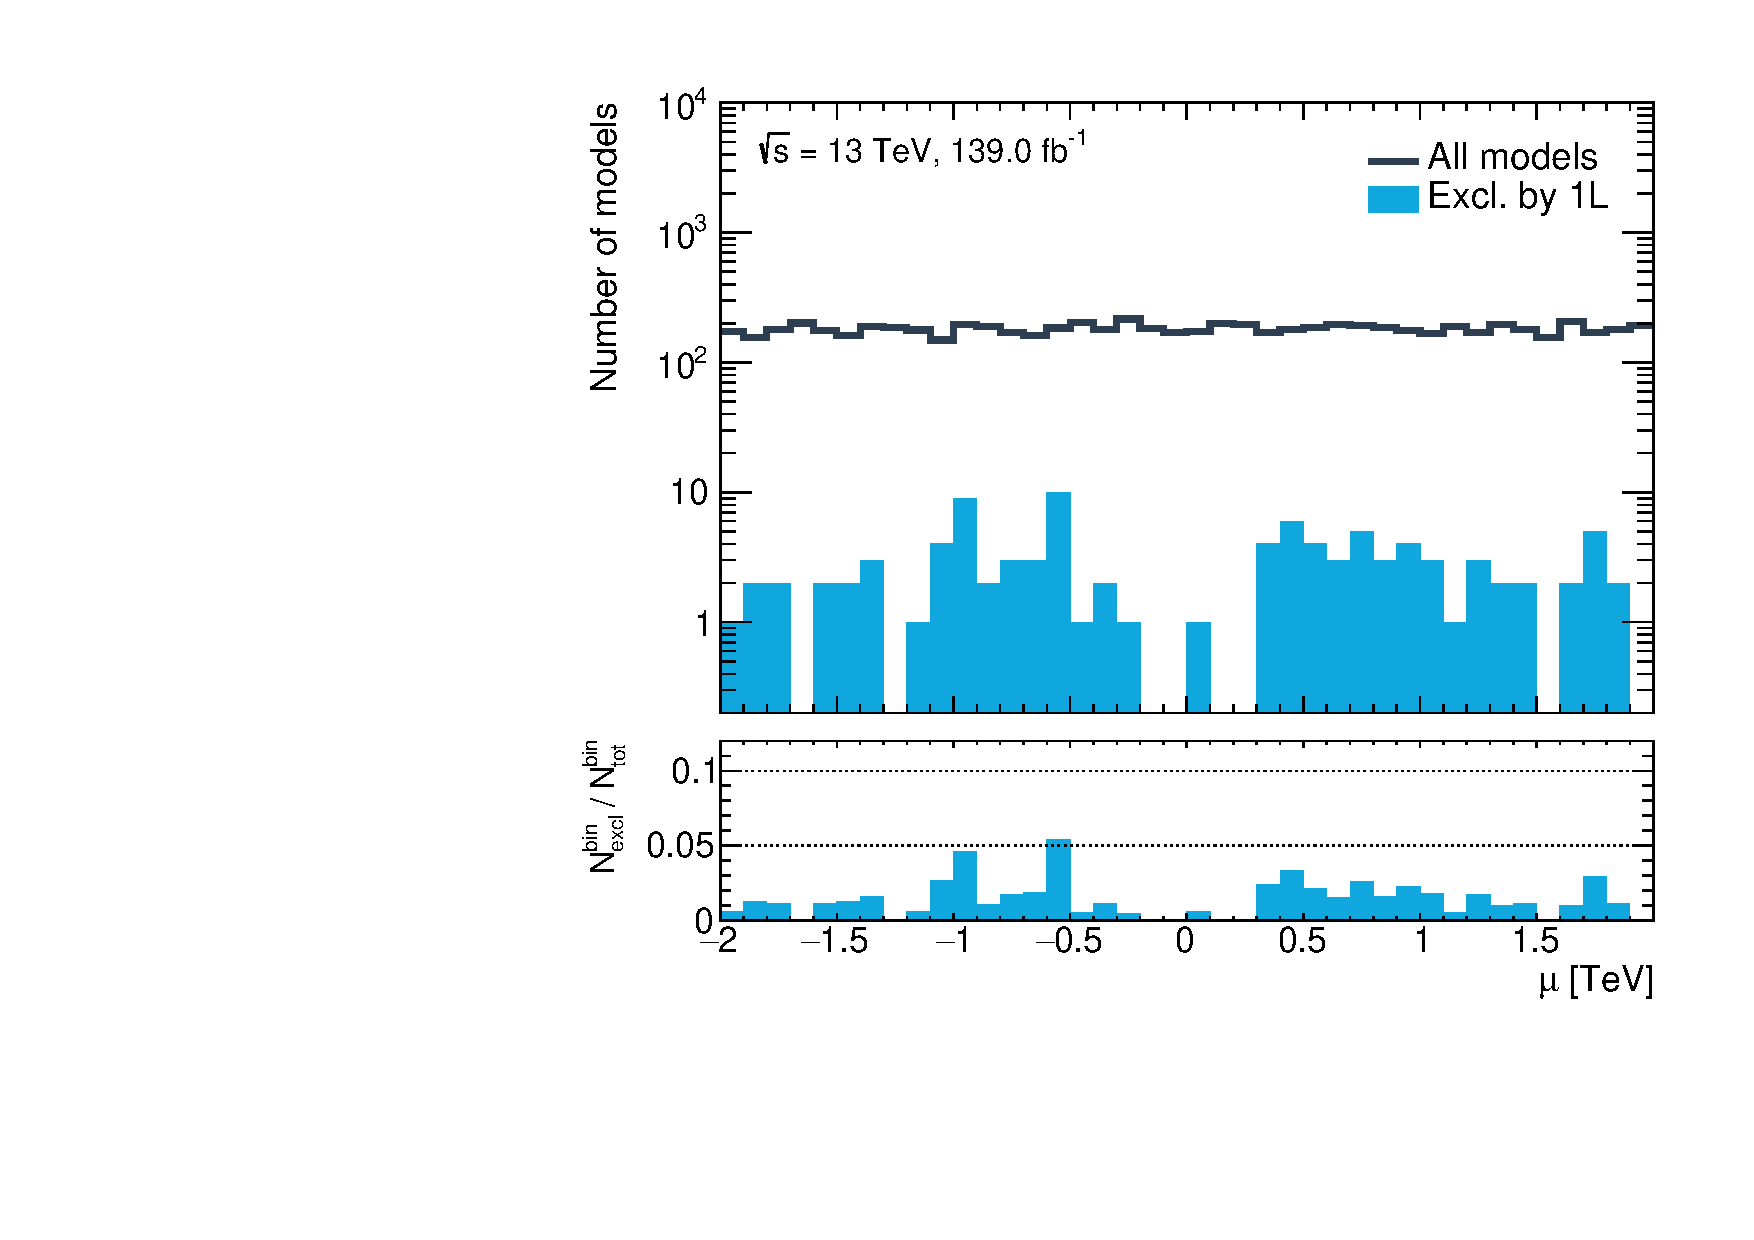
\includegraphics[width=\textwidth]{1D/mu}
	\end{subfigure}\hfill
	\begin{subfigure}[b]{0.5\linewidth}
		\centering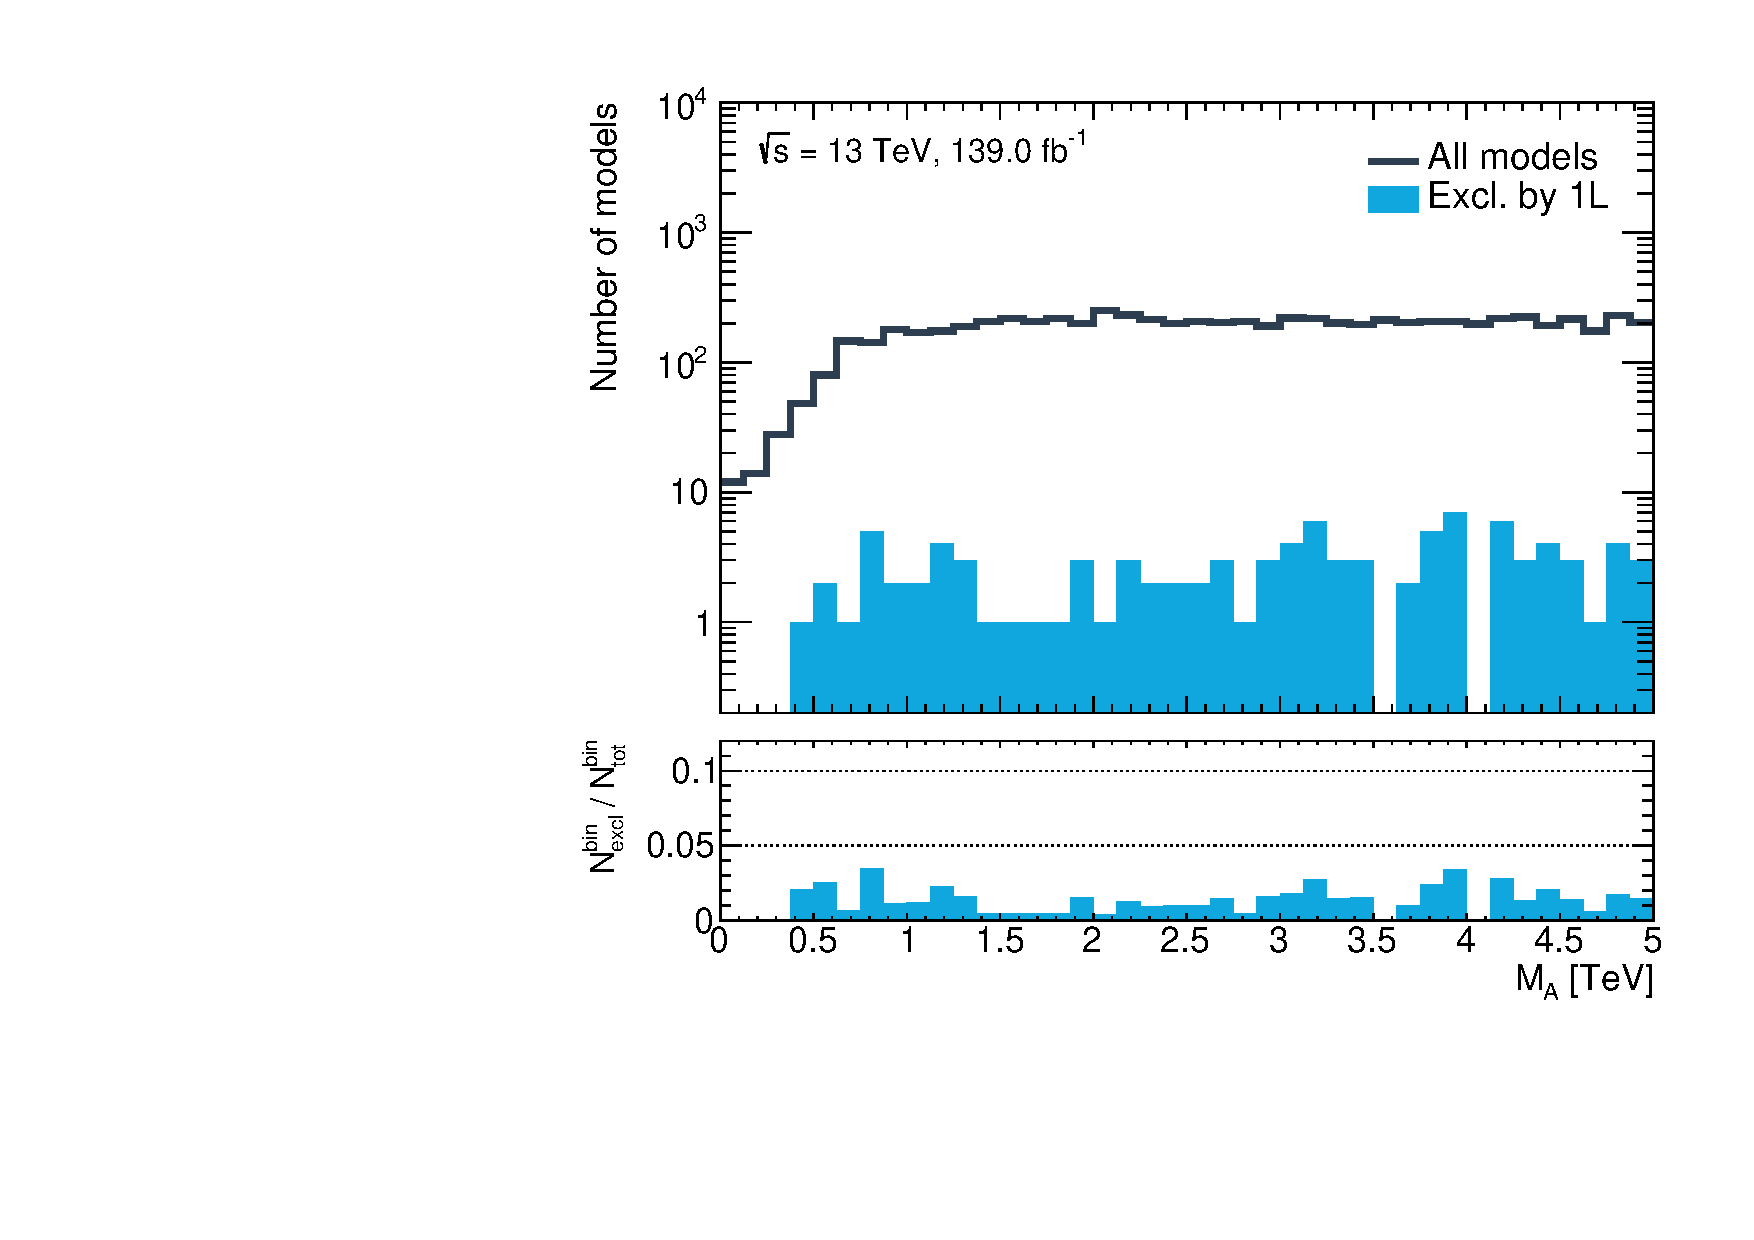
\includegraphics[width=\textwidth]{1D/mA}
	\end{subfigure}\hfill
	\begin{subfigure}[b]{0.5\linewidth}
		\centering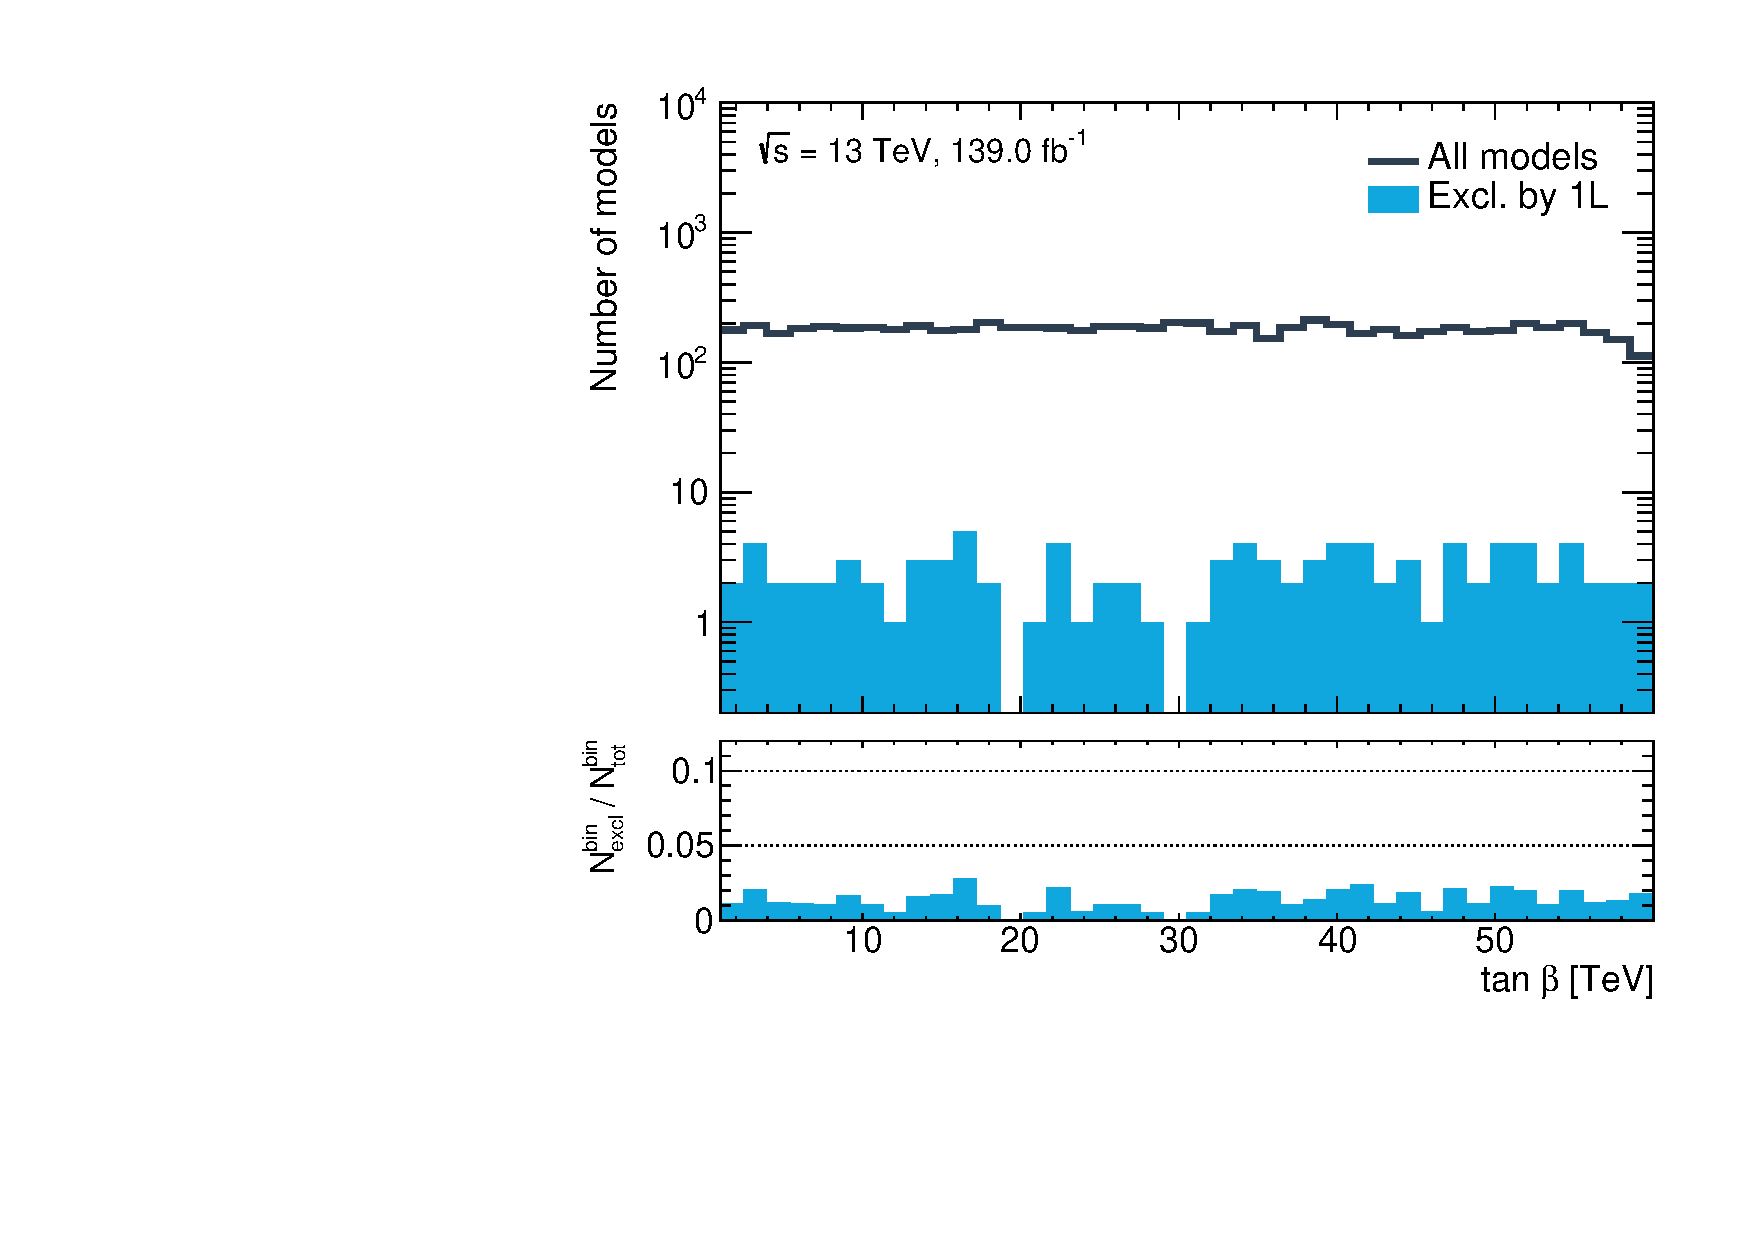
\includegraphics[width=\textwidth]{1D/tanb}
	\end{subfigure}\hfill
	\caption{Bin-by-bin number of excluded models as a one-dimensional function of the \gls{pmssm} parameters sampled relevant to the electroweak sector. The bin-wise fraction of excluded models, $N^\mathrm{bin}_\mathrm{excl} / N^\mathrm{bin}_\mathrm{total}$, is shown in the lower pad. All models are evaluated using the simplified likelihood of the \onelepton search.}
	\label{fig:impact_pMSSM_parameters_1D}
\end{figure}

The impact of the \onelepton search on the \gls{pmssm} parameters relevant to the electroweak sector are shown in one-dimensional distributions in~\cref{fig:impact_pMSSM_parameters_1D}. As already discussed in~\cref{sec:impact_electroweakino_masses}, the \onelepton search has the largest impact for small values in the bino mass parameter $M_1$, leading to models with a bino-like \gls{lsp} when $M_1 < M_2$ and $M_1 \ll \mu$.
Consequently, the proportion of excluded models peaks at slightly higher values in the distribution of the wino mass parameter, $\vert M_2\vert\approx\SI{400}{\GeV}$. As the search is not sensitive to compressed scenarios with a higgsino-like \gls{lsp}, no models with small values in $\vert\mu\vert$ can be excluded. 

Since the pseudoscalar Higgs boson does not directly enter the phenomenology of the models targeted by the \onelepton search, only indirect constraints can be set on $m_\mathrm{A}$, excluding models across the full range of the $m_\mathrm{A}$ distribution sampled.
A similar behaviour is observed in $\tan\beta$ where the excluded models have values of $\tan\beta$ spanning the full range from 1 to 60.
Likewise, no direct constraints on the trilinear scalar couplings ($A_t$, $A_b$, $A_\tau$), and the remaining gluino and third generation squark mass parameters ($M_3$, $m_{\tilde{Q}_3}$, $m_{\tilde{u}_3}$, $m_{\tilde{d}_3}$) is observed, as can be seen from \cref{fig:impact_pMSSM_parameters_1D_2}. 

\improvement{why mA < 500?}

% \begin{figure}
%	\centering
%	\begin{subfigure}[b]{0.5\linewidth}
%		\centering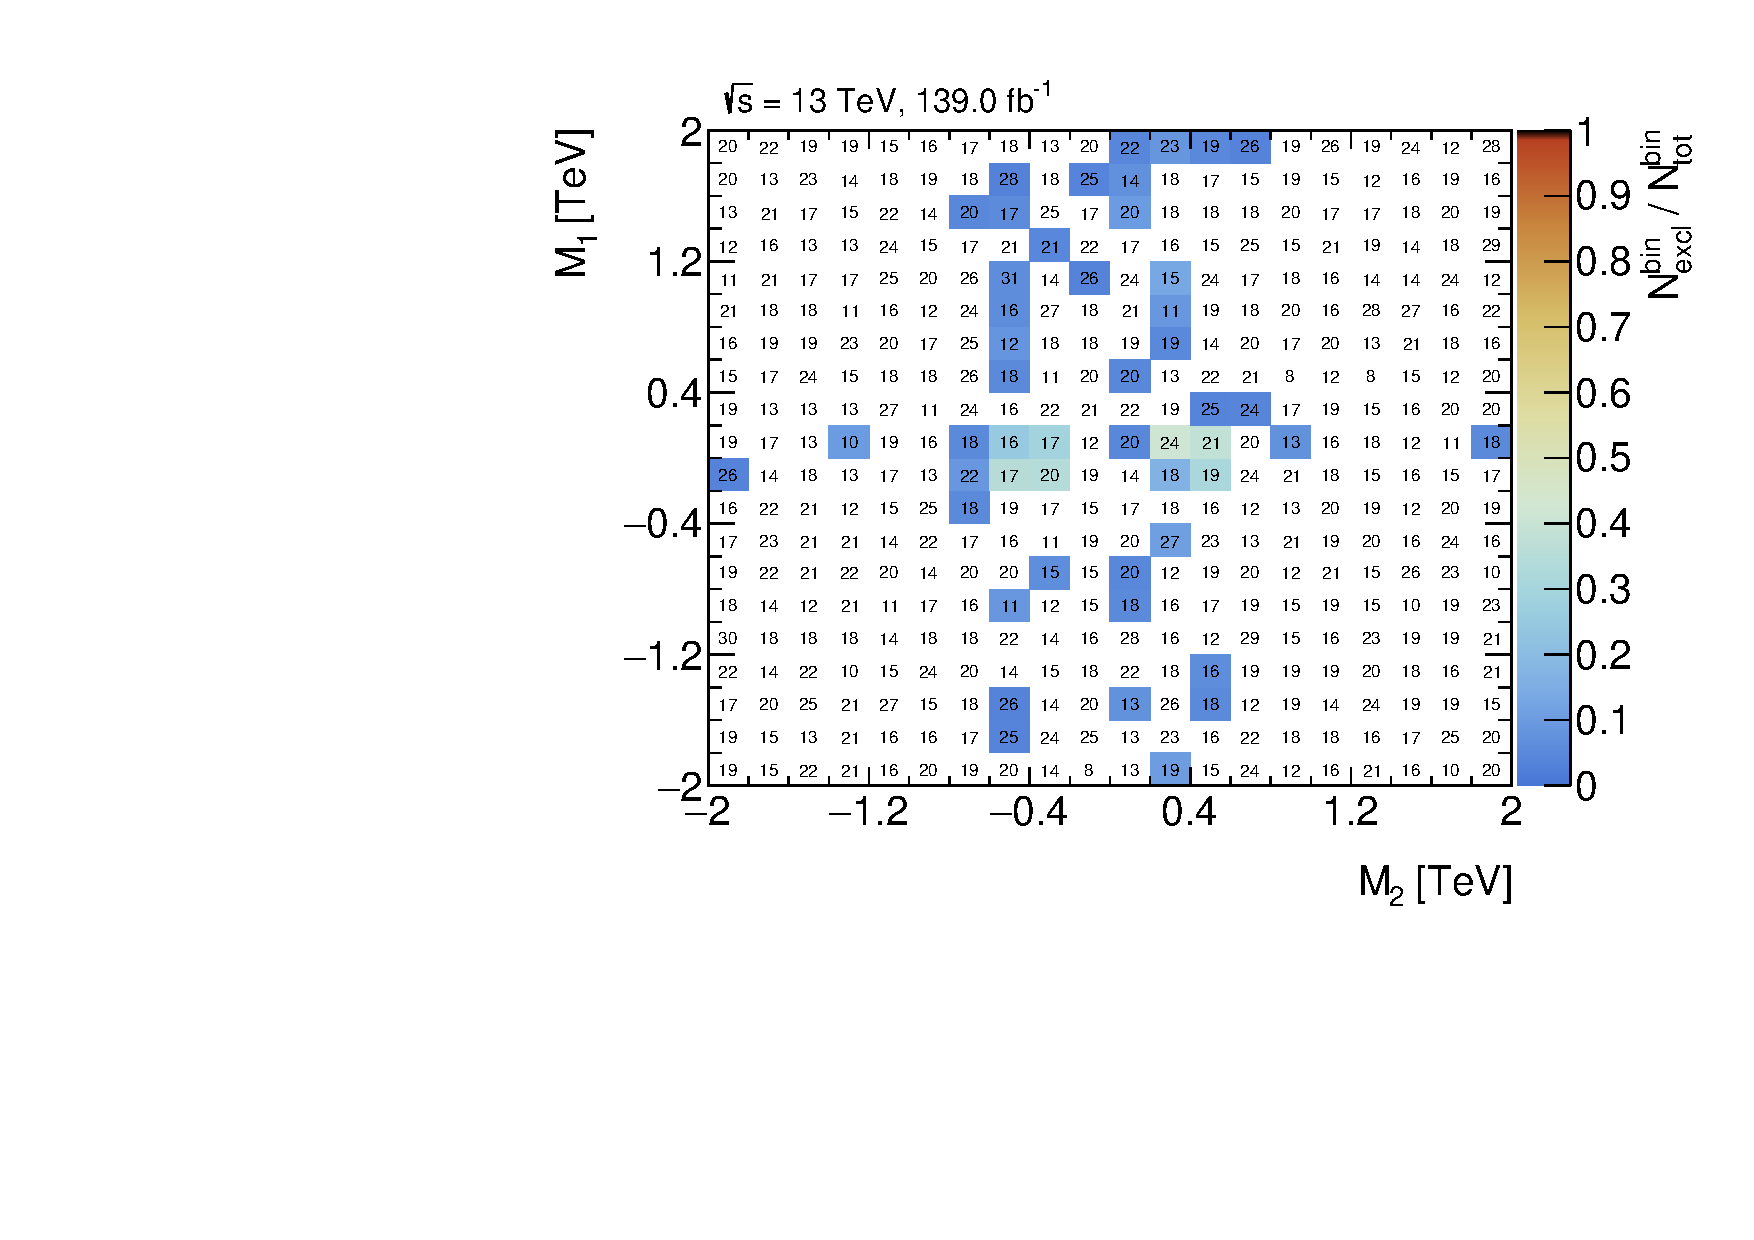
\includegraphics[width=\textwidth]{cut_none/M1_vs_M2}
%		\caption{\label{fig:M1_vs_M2}}
%	\end{subfigure}\hfill
%	\begin{subfigure}[b]{0.5\linewidth}
%		\centering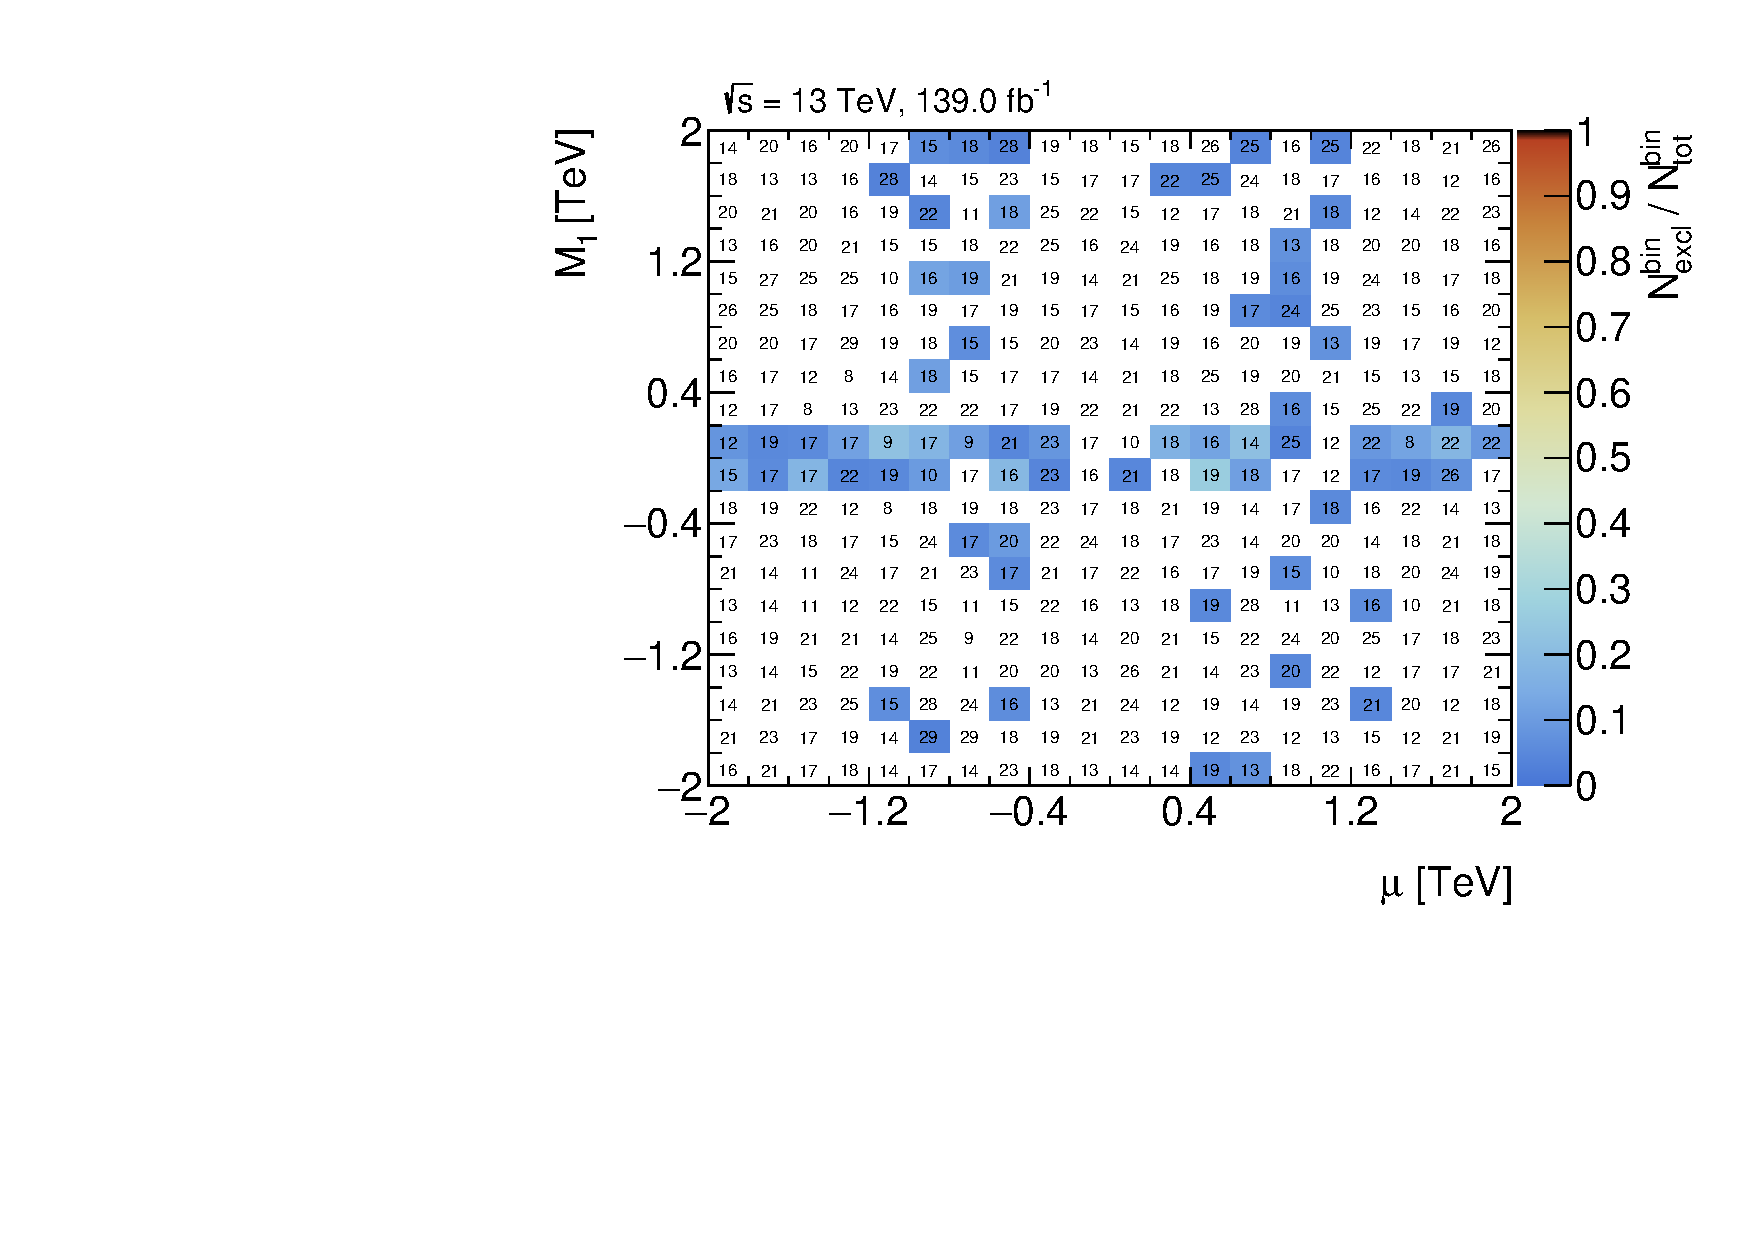
\includegraphics[width=\textwidth]{cut_none/M1_vs_mu}
%		\caption{\label{fig:M1_vs_mu}}
%	\end{subfigure}\hfill
%	\begin{subfigure}[b]{0.5\linewidth}
%		\centering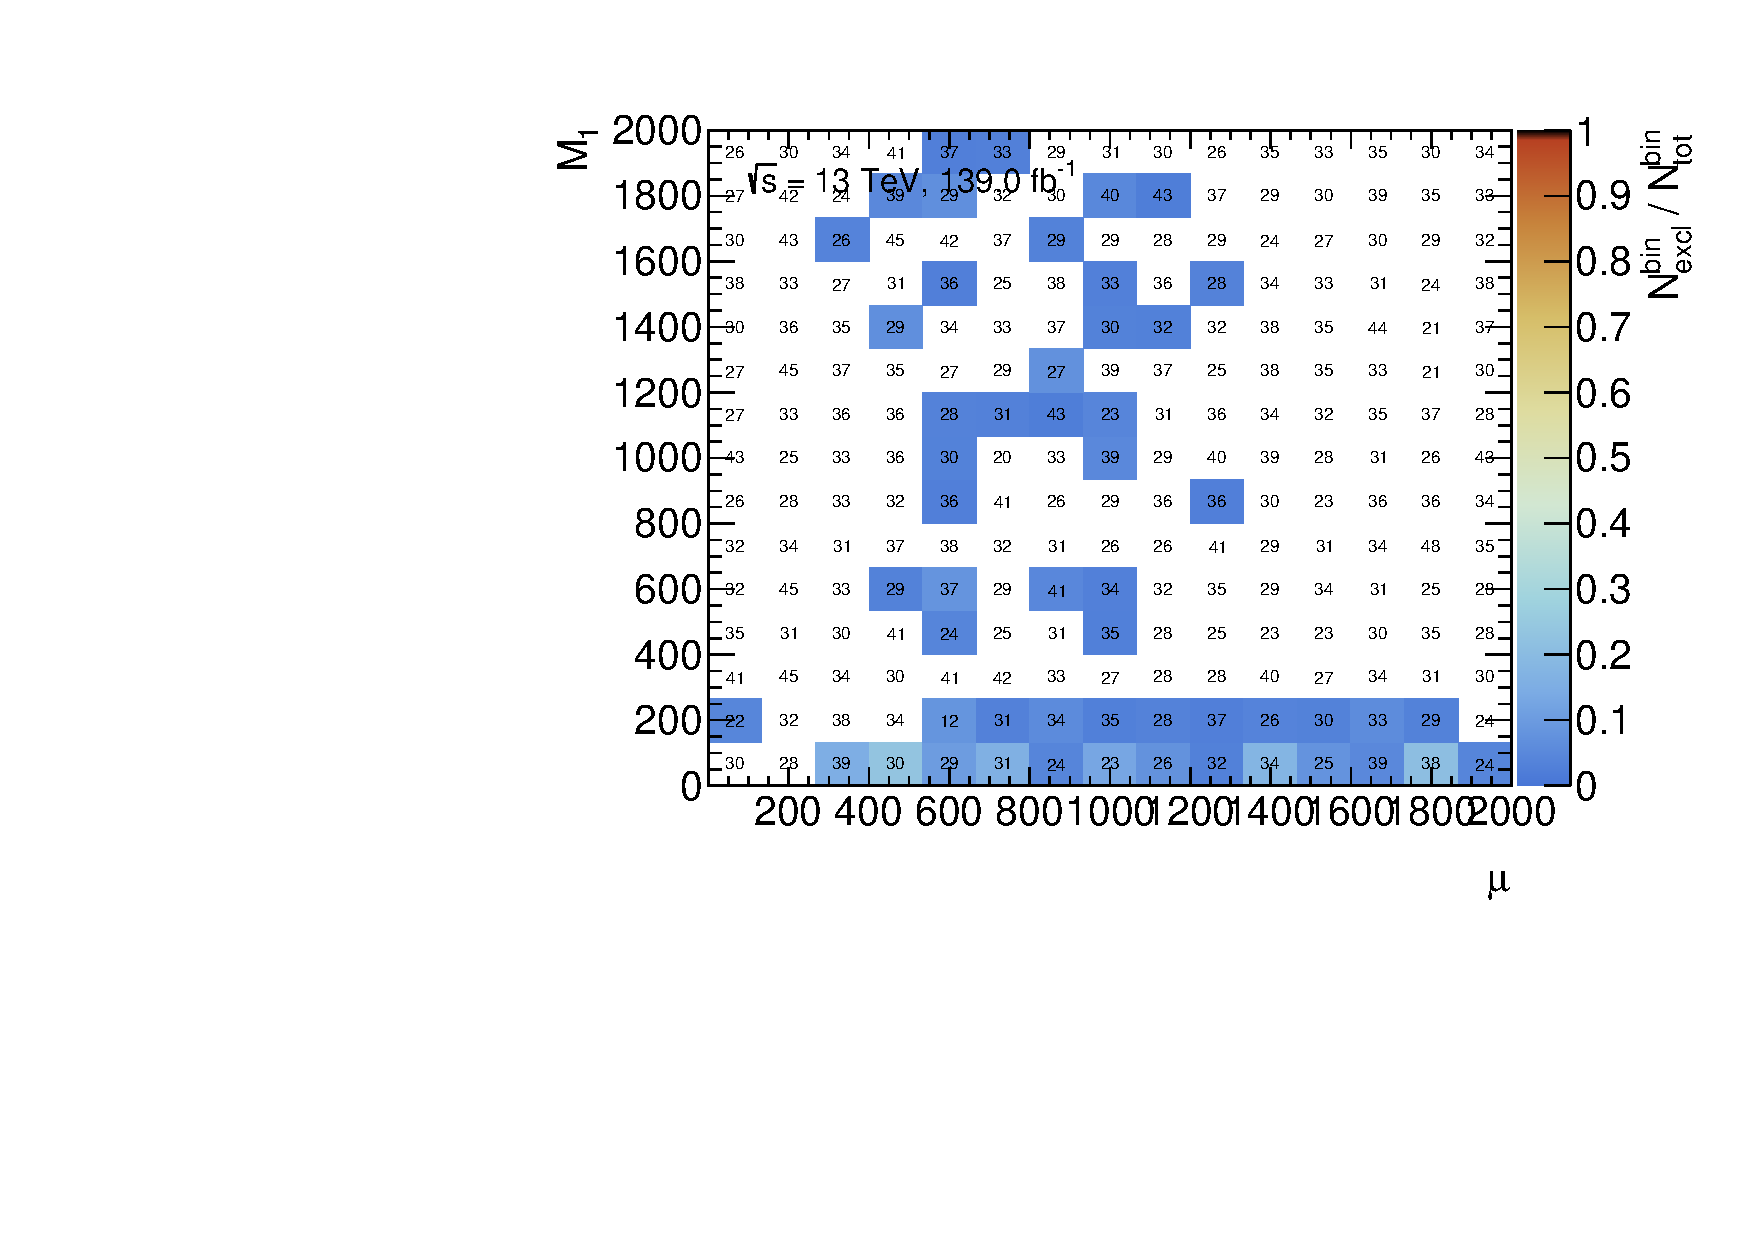
\includegraphics[width=\textwidth]{cut_none/M2_vs_mu}
%		\caption{\label{fig:M2_vs_mu}}
%	\end{subfigure}\hfill
%	\caption{}
%	\label{fig:impact_electroweakinos_2D}
%\end{figure}

\subsection{Impact on dark matter relic density}

 \begin{figure}
	\centering
	\begin{subfigure}[b]{0.445\linewidth}
		\centering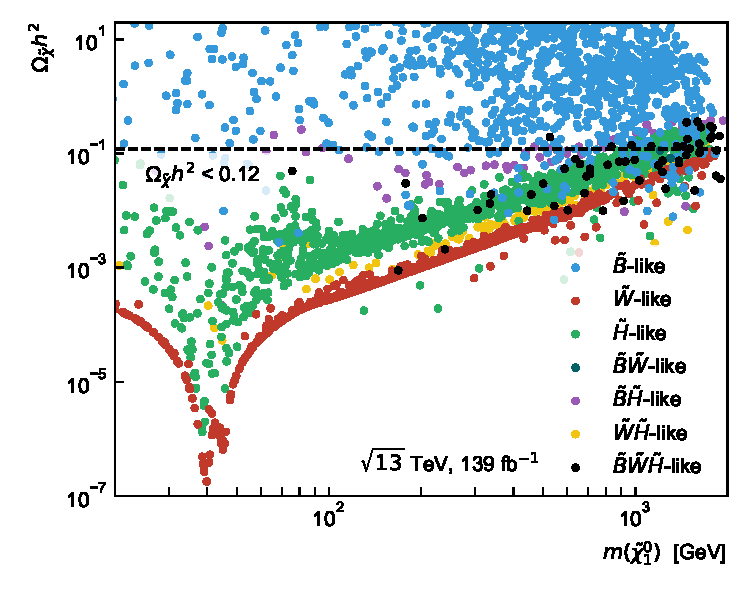
\includegraphics[width=\textwidth]{scatter/relic_density_lsp}
		\caption{\label{fig:relic_density_lsp}}
	\end{subfigure}\hfill
	\begin{subfigure}[b]{0.555\linewidth}
		\centering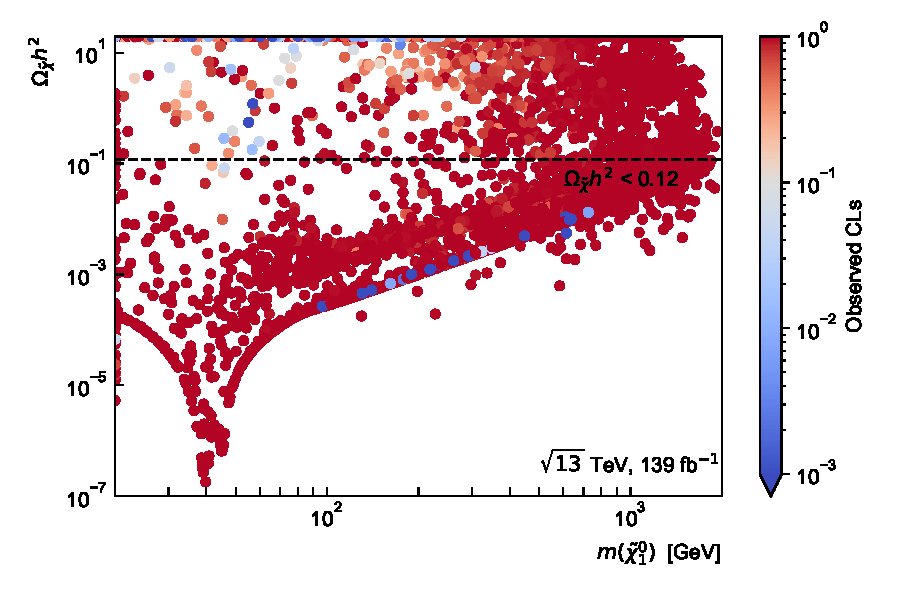
\includegraphics[width=\textwidth]{scatter/relic_density_lsp_cls}
		\caption{\label{fig:relic_density_lsp_cls}}
	\end{subfigure}\hfill
	\caption{Density of the \gls{pmssm} model points sampled in the plane spanned by the relic density and the $\lsp$ mass. The model points are additionally shown as a function of \subref{fig:relic_density_lsp} the nature of their $\lsp$ and \subref{fig:relic_density_lsp_cls} the observed CL$_s$ value obtained for \onethirtynineifb of data using the \onelepton search. The horizontal dashed line represents the \gls{dm} relic density measurement by the Planck collaboration~\cite{Planck}, interpreted as an upper limit $\Omega_{\tilde{\chi}} h^2 < 0.12$ such that the $\lsp$ can be a sub-dominant \gls{dm} component.}
	\label{fig:relic_density}
\end{figure}

The $\lsp$ cosmological abundance, $\Omega_{\tilde{\chi}} h^2$, in dependence of its type and mass is shown in~\cref{fig:relic_density_lsp}. The value of the \gls{dm} relic density measured by the Planck mission is also given~\cite{Planck}. The Planck measurement is interpreted as upper limit on the \gls{dm} relic density, thus allowing the $\lsp$ to be a sub-dominant \gls{dm} component.

Some interesting features are worth highlighting. First, most of the models sampled with a bino-like $\lsp$ result in a cosmological abundance incompatible with the value measured by Planck.
Of the \gls{pmssm} models sampled in this thesis, only models with a $\lsp$ containing a considerable wino or higgsino component satisfy $\Omega_{\tilde{\chi}} h^2 < 0.12$ over a large range of $m(\lsp)$.
Models with $m(\lsp) \simeq m(Z)/2$ produce especially low values in $\Omega_{\tilde{\chi}} h^2$ as the $\lsp$ can resonantly annihilate through \textit{s}-channel $Z$ exchange. This is the so-called \textit{Z-funnel}, a mechanism that becomes more efficient, the larger the higgsino component of the $\lsp$ is~\cite{Cabrera:2016wwr}.
A similar funnel exists around $m(h)/2$ but is not visible in~\cref{fig:relic_density_lsp}. An additional resonant mechanism can however be seen: co-annihilation of a nearly mass-degenerate $\charg\lsp$ pair at $m(W)/2$ through \textit{s}-channel \textit{W} exchange.\unsure{is this correct?}

In practice, the \gls{lep} limits\footnote{In models where the mass difference between $\charg$ and $\lsp$ is small, the limit on the chargino mass by \gls{lep} is only $m(\charg) > \SI{92}{\GeV}$~\cite{lep_susy_results}.} on the chargino mass of $\charg > \SI{103.5}{\GeV}$~\cite{lep_susy_results} rule out models with $\vert M_2 \vert \lesssim \SI{100}{\GeV}$ and $\vert \mu \vert \lesssim \SI{100}{\GeV}$, leaving only models with a bino-like \gls{lsp} in the region with $m(\lsp)\lesssim \SI{100}{\GeV}$.

Although theoretically models with a bino-like $\lsp$ could produce low $\lsp$ relic density values through the $Z$- and $h$-funnels, in practice such models are not sampled in this thesis due to the sampling technique used.
In order to further study the impact of the \onelepton search on models relevant to the \gls{dm} phenomenology, \ie models with a bino-like \gls{lsp} in the $Z$- and $h$-funnels, a different sampling technique would need to be employed, including experimental constraints in the sampling priors in addition to oversampling models with a bino-like \gls{lsp}.
%For this reason, in this work, only a very small number of models with a bino-like $\lsp$ with $m(\lsp) \lesssim \SI{100}{\GeV}$ have a relic density compatible with the Planck measurement.
%Oversampling this region should however still reveal the typical $Z$- and $h$-funnels for models with a bino-like \gls{lsp}~\cite{pMSSM-scan-run1:2015baa,Aaboud:2016wna}.
%If the $\charg/\neutr$ masses of such models fall into the range where the \onelepton search is sensitive,\ie $\charg\neutr$ pair-production has high enough cross section, the \onelepton search can be excepted to exclude a sizeable fraction of these models, thus warranting additional, dedicated scans using experimental constraints in the sampling priors. 

Although of limited use due to the limited number of models in the relevant parameter space, the impact of the \onelepton search on the \gls{dm} relic density can still be investigated with the models available. \Cref{fig:relic_density_lsp_cls} shows the $\lsp$ cosmological abundance in dependence of its mass. Instead of encoding the nature of the $\lsp$, the colour now encodes the observed CL$_s$ value obtained by the \onelepton search. By comparing with \cref{fig:relic_density_lsp}, it can be seen that the majority of the models with a bino-like $\lsp$, excluded by the \onelepton search, have a cosmological abundance not satisfying $\Omega_{\tilde{\chi}} h^2 < 0.12$. Through its limited sensitivity to some of the models with a wino-like $\lsp$, the \onelepton search is, however, still able to exclude some models with a compatible \gls{lsp} relic density. 

\section{Discussion}

Large-scale reinterpretations in high-dimensional \gls{susy} model spaces are crucial in order to assess the sensitivity of \gls{susy} searches in the context of realistic \gls{susy} scenarios. The evaluation of signal models at smeared truth level, in combination with the simplified likelihoods introduced in~\cref{ch:simplify}, offers a computationally efficient but still reliable approach for such reinterpretations.

A reinterpretation of the \onelepton search in a limited number of models sampled from the \gls{pmssm} with a focus on the electroweak sector revealed that the search is sensitive to \gls{susy} scenarios beyond the canonical simplified model originally considered.
In general, the simplified model phenomenology maps reasonably well onto a portion of the \gls{pmssm} parameter space. The sensitivity of the \onelepton search towards \gls{pmssm} models is, however, negatively impacted by the competing decays $\neutr \rightarrow Z \lsp$ and $\neutr \rightarrow h \lsp$, breaking one of the main assumptions of the simplified model.
In order to maximise the sensitivity of future searches to $\charg\neutr$ pair-production in more complete \gls{susy} scenarios, it is therefore crucial to target both decay modes at the same time.
In searches targeting final states with one lepton, multiple jets and missing transverse momentum, both the \textit{b}-jet multiplicity as well as the invariant mass of the jets originating from the decays $h\rightarrow b\bar{b}$ and $Z\rightarrow q\bar{q}$ can easily be exploited to develop disjoint\footnote{Building signal regions that are not orthogonal to each other prevents the construction of a single likelihood and thus does not allow statistical combination.} signal regions targeting both decay modes.

Beyond the combination of single decay modes, it could be worth targeting not only $\charg\neutr$ production, but also the $\charg\charg$ production mode at the same time in a single likelihood function. In ATLAS, work is for example ongoing to perform a search for electroweakinos in the \onelepton final state using dedicated signal regions targeting both $\charg\neutr \rightarrow WZ\lsp\lsp\rightarrow \ell\nu_\ell q\bar{q} \lsp\lsp$ and $\charg\charg \rightarrow WW\lsp\lsp\rightarrow \ell\nu_\ell q\bar{q}' \lsp\lsp$ at the same time. 

Finally, the impact of the \onelepton search on the \gls{dm} relic density was discussed. The parameter ranges and sampling technique chosen were used to guarantee the scan to be as general as possible. For this reason, many models sampled are not directly relevant to the \gls{dm} phenomenology. Only a small number of models with a bino-like $\lsp$ are sampled from $Z$- and $h$-funnel region where $\Omega_{\tilde{\chi}} h^2 < 0.12$ is satisfied. Outside of these two funnels, models with a bino-like $\lsp$ only satisfy the relic density constraint for $\charg$ and $\lsp$ masses outside of the parameter space that the \onelepton search is sensitive to. In order to be able to further investigate the impact of the \onelepton search on \gls{dm} observables---especially in the $Z$ and $h$-funnels---a different sampling technique would need to be adopted, including experimental constraints in the sampling priors and oversampling the relevant regions of the parameter space. 



